%   % !TEX root = ../../VIII,3_Rahmen-TeX_8-1.tex
%
%
%   Band VIII, 3		Rubrik STOSS
%
%   Signatur/Tex-Datei:	LH_37_05_104-105
%
%   RK-Nr. 	60323
%
%   \ref{RK60323}
%
%   Überschrift: 	Physico-Mechanicae leges ex congressu corporum ductae
%   
%   Unterrubrik:			Kinematik? Überblick?
%
%   Datierung:		Herbst 1688
%
%   edlabels:			(zahlreiche)
%
%   Diagramme: 		5 
%
%
%   NB: 						(Anmerkungen)					??
%
%
%
\selectlanguage{ngerman}
\frenchspacing
%
\begin{ledgroupsized}[r]{120mm}
\footnotesize
\pstart
\noindent\textbf{Überlieferung:}
\pend
\end{ledgroupsized}
%
\begin{ledgroupsized}[r]{114mm}
\footnotesize
\pstart \parindent -6mm
\makebox[6mm][l]{\textit{L}}%
Konzept:
LH~XXXVII~5, Bl.~104\textendash105.
Ein Bogen~4\textsuperscript{o};
oberer Rand beschnitten, die übrigen ausgefranst;
Papiererhaltungsmaßnahmen.
Vier Seiten.
\pend
\end{ledgroupsized}
%
%
\vspace{5mm}
\begin{ledgroup}
\footnotesize
\pstart
\noindent%
\textbf{Datierungsgründe:}
Der vorliegende Entwurf N.~\ref{RK60323} \textit{Physico-mechanicae leges ex congressu corporum ductae} besteht aus zwei inhaltlich verschiedenen Teilen.
Im ersten (bis S.~\refpassage{LH_37_05_104v_scwitch-2}{LH_37_05_104v_scwitch-2}) werden die Gesetze des direkten zentralen Stoßes zweier elastischer Körper aufgestellt.
Im zweiten Teil werden einige dieser Gesetze in Anspruch genommen, um die Veränderung der Geschwindigkeit eines Körpers zu berechnen, der sich durch ein widerstehendes Medium bewegt.
Bei dieser Berechnung stützt sich Leibniz auf die physikalische Annahme, dass die Veränderung der Geschwindigkeit von mikroskopischen Stößen herrührt, die zwischen dem beweglichen Körper und den Teilchen (\textit{corpuscula}) des Mediums erfolgen.
Unter der zusätzlichen Annahme, dass das Medium selbst bewegt ist, erklären die mikroskopischen Stöße aus Leibnizens Sicht nicht nur die Verzögerung des beweglichen Körpers (durch Reibung), sondern auch dessen Beschleunigung (durch Gravitation) \textendash\ womit Galileis\protect\index{Namensregister}{\textso{Galilei} (Galilaeus, Galileus), Galileo 1564\textendash1642}
Lehre vom freien Fall in ihrer Gesamtheit bestätigt sein soll.
%Die Annahme mikroskpischer Stöße soll am Ende von N.~\ref{RK60323} offenbar auch dazu dienen, die Zergliederung einer Umlaufbahn in eine inertielle und eine zentripetale Bewegung zu begründen, was schließlich die Aufmerksamkeit auf .
Dieses in seinen Grundzügen auf die \textit{Hypothesis physica nova}\cite{00256} (1671) zurückgehende Erklärungsmodell hatte Leibniz vornehmlich in Paris (1675) entwickelt, wie zahlreiche in \textit{LSB} VIII,~2 edierte Texte zeigen.
\pend\pstart
Die \textit{Physico-mechanicae leges} bauen inhaltlich auf dem zwischen Ende Oktober 1686 und Anfang Februar 1687 verfassten Entwurf N.~\ref{RK41201} \textit{Leges concursuum} auf.
Der erste Teil von N.~\ref{RK60323} ist wesentlich eine (streckenweise sehr getreue) Wiedergabe der Ergebnisse, zu denen die Untersuchung über die Stoßgesetze in N.~\ref{RK41201} geführt hat.
Die Ähnlichkeit beider Texte ist zuweilen so weitgehend, dass als Zwischenvorlage zur Anfertigung von N.~\ref{RK60323} das nicht weiter ermittelte \glqq Handbuch\grqq\ anzunehmen ist, auf das Leibniz selbst hindeutet (vgl. N.~\ref{RK60323}, S.~\refpassage{LH_37_05_104r_enchiridion_yfj-1}{LH_37_05_104r_enchiridion_yfj-2}; N.~\ref{RK41201}, Randbemerkung zu S.~\refpassage{LH_35_09_21_001r_manuale_obrrnd-1}{LH_35_09_21_001r_manuale_obrrnd-2}).
Der Terminus post quem für die Datierung der \textit{Physico mechanicae leges} ergibt sich jedoch vielmehr aus der Besprechung des ersten Lehrsatzes aus Newtons%
\protect\index{Namensregister}{\textso{Newton} (Neutonus), Isaac 1643\textendash1727}
\textit{Principia}\cite{00535} im zweiten Teil des Entwurfes (vgl. N.~\ref{RK60323}, S.~\refpassage{LH_37_05_105v_PhNPM_Stelle-1}{LH_37_05_105v_PhNPM_Beweis-2}).
Leibniz erkennt dort, dass Newtons\protect\index{Namensregister}{\textso{Newton} (Neutonus), Isaac 1643\textendash1727}
Lehrsatz eine Verallgemeinerung von Keplers\protect\index{Namensregister}{\textso{Kepler} (Keplerus), Johannes 1571\textendash1630}
zweitem Planetengesetz ist (S.~\refpassage{LH_37_05_105v_PhNPM_Stelle-1}{LH_37_05_105v_PhNPM_Stelle-2}), fasst den Beweis des Satzes sorgfältig zusammen (S.~\refpassage{LH_37_05_105v_PhNPM_Beweis-1}{LH_37_05_105v_PhNPM_Beweis-2}) und gibt das zugehörige Diagramm nur teilweise, aber hinreichend getreu wieder (S.~\pageref{LH_37_05_105v_Fig.3}, \lbrack\textit{Fig.~3}\rbrack).
Aus diesen Gründen ist auszuschließen, dass die Rezension\cite{01356} der \textit{Principia},\cite{00535} die C.~Pfautz\protect\index{Namensregister}{\textso{Pfautz} (Pfauzius), Christoph 1645\textendash1711}
in den \textit{Acta eruditorum} (Juni 1688, S.~303\textendash315) veröffentlicht und Leibniz exzerpiert hatte (vgl. LH~XXXV~10, 7 Bl.~13\textendash14), die unmittelbare Quelle von Leibnizens Referat gewesen sein kann, welches vielmehr aus einer eigenständigen Lektüre von Newtons\protect\index{Namensregister}{\textso{Newton} (Neutonus), Isaac 1643\textendash1727}
Abhandlung hervorgegangen sein muss.
Leibnizens erste bezeugte Lektüre der \textit{Principia}\cite{00535} fand \textendash\ wie \textsc{Bertoloni Meli} 1993 (S.~97)\cite{01357}
% D.~Bertoloni Meli (\textit{Equivalence and Priority}, Oxford 1993, S.~97\cite{01357}) 
nachgewiesen hat \textendash\ im Herbst 1688 statt, als Leibniz sich auf dem Weg nach Italien in Wien aufhielt.
Folglich kann auch der Entwurf N.~\ref{RK60323} nicht vor dem Herbst 1688 verfasst worden sein.
Zur Bestätigung sei bemerkt, dass aus dieser wohl ersten Lektüre der \textit{Principia}\cite{00535} Auszüge entstanden sind (LH XXXV~10, 7 Bl.~32\textendash35), die ausführlich auf die in N.~\ref{RK60323} besprochene Stelle eingehen (vgl. \textsc{Bertoloni Meli} 1993 S.~230\textendash232, Z.~295\textendash383\cite{01357}).% Bertoloni Meli, \textit{Equivalence and Priority}, S.~230\textendash232, Z.~295\textendash383\cite{01357}
\pend%
%
\pstart%
Da Leibniz nach seiner Abfahrt aus Wien im Februar 1689 keineswegs aufgehört hat, sich ausführlich mit Newtons%
\protect\index{Namensregister}{\textso{Newton} (Neutonus), Isaac 1643\textendash1727}
\textit{Principia}\cite{00535} zu befassen, könnte der Entwurf N.~\ref{RK60323} auch später verfasst worden sein.
Gegen dessen Entstehung nach Ende 1688 sprechen jedoch folgende Gründe:
\pend%
\newpage
\pstart%
(1) Die Auseinandersetzung mit den \textit{Principia}\cite{00535} hat Leibniz monatelang begleitet und zahlreiche Spuren in seinen Handschriften hinterlassen: Neben den erwähnten Auszügen sind zahlreiche weitere eigenständige Entwürfe erhalten, die im Herbst 1688 oder Anfang 1689 in Wien niedergeschrieben wurden, sowie spätere, in Rom verfasste Auszüge und die Marginalien im Leibnizens Handexemplar (siehe die Liste in \textsc{Bertoloni Meli} 1993, S.~308\,f.; diese Texte werden größtenteils voraussichtlich % \textendash\ mit Ausnahme der Marginalien \textendash\ 
in künftigen Bänden von \textit{LSB} VIII ediert).
Der Entwurf N.~\ref{RK60323} dürfte noch ganz am Anfang dieser Entwicklung sein, wenn Leibniz dort bei der Besprechung des ersten Lehrsatzes aus den \textit{Principia}\cite{00535} ausführlich vermerkt:
\textit{Haec ergo examinare ex principiis nostris magnum operae pretium erit}
(S.~\refpassage{LH_37_05_105v_ohjelma-1}{LH_37_05_105v_ohjelma-2}).
\pend%
%
\pstart%
(2) Im Zusammenhang mit seiner Auseinandersetzung mit Newtons%
\protect\index{Namensregister}{\textso{Newton} (Neutonus), Isaac 1643\textendash1727}
\textit{Principia}\cite{00535} veröffentlichte Leibniz drei Aufsätze in den \textit{Acta eruditorum}: Im Januarheft \textit{De lineis opticis} (S.~36\textendash38)\cite{01358} und \textit{Schediasma de resistentia medii et motu projectorum in medio resistente} (S.~38\textendash47, \textit{LMG} VI, S.~135\textendash143);\cite{01024}
im Februarheft \textit{Tentamen de motuum coelestium causis} (S.~82\textendash96, \textit{LMG} VI, S.~144\textendash161;\cite{00543} diese Aufsätze werden voraussichtlich in künftigen Bänden von \textit{LSB} VIII ediert).
Die thematische Verwandtschaft zwischen dem zweiten Teil von N.~\ref{RK60323} und dem (in N.~\ref{RK60323} nie erwähnten) \textit{Schediasma},\cite{01024} kündigt sich bereits im Titel des veröffentlichten Aufsatzes an.
Hierbei ist jedoch zu bemerken, dass im \textit{Schediasma}\cite{01024} nur noch die Verzögerung eines sich in einem widerstehenden Medium bewegenden Körpers behandelt wird, während die Betrachtung des Mediums als Ursache der Gravitation und der Beschleunigung fallender Körper nicht mehr vorkommt (sie ist in das etwas später veröffentlichte \textit{Tentamen}\cite{00543} ausgewandert, wo Leibniz sie im Rahmen seiner Theorie der Planetenbewegung entfaltet).
Der Umstand, dass beide später getrennt behandelte Themen \textendash\ das Medium als Ursache der Verzögerung und das Medium als Ursache der Beschleunigung \textendash\ im Entwurf N.~\ref{RK60323} noch zusammen und ohne Bezüge auf Leibnizens einschlägige Veröffentlichungen vom Anfang 1689 behandelt werden, ist wohl als Zeichen für eine frühere Entstehung zu deuten.
\pend%
%
\pstart%
(3) 
%Im zweiten Teil von N.~\ref{RK60323} erwähnt Leibniz nebenbei, auch \glqq anderwoher\grqq\ (\textit{aliunde}) ergebe sich, dass die Verzögerung eines Körpers durch den Widerstand des Mediums von der Geschwindigkeit abhängig sei (S.~\refpassage{LH_37_05_105r_aliunde-1}{LH_37_05_105r_aliunde-2}).
%Damit spielt er möglicherweise auf die 
Eine umfangreiche Untersuchung über die dissipative Wirkung eines widerstehenden Mediums hatte Leibniz bereits im Jahr 1675 in Paris angestellt (siehe \textit{LSB} VIII,~2 N.~30 bis N.~38).
Ein wichtiges Ergebnis dieser Untersuchung war die Feststellung gewesen, dass von einem fluiden Medium zwei Widerstandsarten hervorgehen: ein \textit{absoluter} Widerstand, der von der Geschwindigkeit des beweglichen Körpers unabhängig sei, und ein geschwindigkeitsabhängiger \textit{relativer} Widerstand % \textendash\ wobei sich die Verzögerung schließlich in beiden Fällen als proportional zur Geschwindigkeit erweise 
(vgl. VIII,~2 N.~34\textsubscript{4}; N.~35; N.~36\textsubscript{1}; N.~36\textsubscript{2}).\cite{01368}\cite{01369}\cite{01370}\cite{01371}
Diese für Leibnizens Reibungslehre grundlegende Unterscheidung, % zweier Arten des Widerstands, 
die noch im \textit{Schediasma de resistentia medii}\cite{01024} vom Januar 1689 die zentrale Rolle spielen sollte, bleibt im zweiten Teil des Entwurfs N.~\ref{RK60323} unerwähnt.
Auch dieser Umstand dürfte darauf hindeuten, dass N.~\ref{RK60323} vor dem \textit{Schediasma}\cite{01024} entstand.
Als Leibniz dieses letztere zu einem späteren Zeitpunkt (jedenfalls noch vor Ende 1688) anfertigte, knüpfte er offenbar an die Ergebnisse seiner Pariser Untersuchung an und baute sie weitgehend aus, während sie bei der Abfassung von N.~\ref{RK60323} noch unberücksichtigt geblieben waren.
\pend%
%
\pstart%
Insgesamt sind die \textit{Physico-mechanicae leges} N.~\ref{RK60323} folglich auf den Herbst 1688 zu datieren.
Ihre Anfertigung muss nach Leibnizens wohl erster Lektüre von Newtons%
\protect\index{Namensregister}{\textso{Newton} (Neutonus), Isaac 1643\textendash1727}
\textit{Principia}\cite{00535} erfolgt sein und fand höchstwahrscheinlich noch vor der Abfassung des \textit{Schediasma de resistentia medii}\cite{01024} statt, das im Januar 1689 veröffentlicht wurde.
\pend%
%\vspace{1.0em}%
%%
%\pstart
%Wegen Verweis auf Newton (auf Bl.~105~v\textsuperscript{o}: Newton ,illustravit‘ Keplers 2. Gesetz; Verwendung des Begriffs ,vis centripeta‘) ist zunächst 1687 als terminus post quem anzunehmen. Wegen der nachfolgenden Umständen vielmehr \textbf{Sommer bzw.\ Herbst 1688}:
%\pend
%%
%\pstart
%Nach heutigem Kenntnisstand beginnt Leibnizens Auseinandersetzung mit den \textit{Principia} erst mit der Lektüre der Rezension (Pfautz) in den \textit{Acta Eruditorum} vom Juni 1688, S.~303\textendash315. Davon sind Auszüge von L überliefert (LH XXXV 10, 7 Bl.~13\textendash14, RK 60041). Leibniz hat im Prioritätsstreit die Lektüre der Rezension nie bestritten.
%%
%Zudem hat Bertoloni Meli (1993) nachgewiesen, dass L bereits im Herbst 1688 in Wien die \textit{Principia} las (Auszüge mit Bemerkungen = LH XXXV 10, 7 Bl.~32\textendash35, RK 57065, ediert in Bertoloni Meli 1993, S.~220\textendash236), und nicht erst ab April 1689 in Rom, wie Leibniz im Prioritätsstreit behauptete.
%\pend
%\pstart
%\textbf{Offene Frage}: Inwiefern setzt dieses Stück die Lektüre der \textit{Principia} voraus (im Gegensatz zur bloßen Rezension)? Die Rezension nennt den Begriff \textit{vis centripeta} (S.~305) und Keplers 2.\ Gesetz (S.~310).%
%\pend
%%
%\pstart
%Auch in N.~\ref{RK60038} verwendet Leibniz den Ausdruck \glqq quantitas centripeta vel centrifuga\grqq.%
%\pend
%%
%\pstart
%\textbf{Weitere offene, datierungsrelevante Frage}: Welches Verhältnis zur Schrift \textit{Schediasma de resistentia medii}? Welches Verhältnis (bzw. gar keins) hat das Stück zu Huygens' mechanistische (und damit Leibniz-affine) Theorie der (Planeten-)Bewegung in einem Medium, welche um 1690 erschien? (\textit{Traité de la Lumière/Cause de la pesanteur}, vgl. Leibnizens Auszug N.~\ref{RK58948} und andere Stücke.)
%\pend
%%
%\pstart
%\textbf{Frage der Unterrubrikzuweisung:} Denkbar wäre die Zuweisung zur UR \glqq Kinematik\grqq. Nur entfernt böten sich die Rubriken \glqq Krafterhaltung\grqq\ oder \glqq Schiefer Stoß\grqq\ an (letztere wird wohl ohnehin aufgelöst). Begründung:
%\\ Erstens: Das Stück hat, wie bereits festgestellt, einige Ähnlichkeiten oder zumindest eine entstehungsgeschichtliche Verbindung mit N.~\ref{RK41201} \glqq Leges concursuum\grqq\ (Mitte 80er Jahre; Stichwort \textit{Enchiridium / Manuale}). N.~\ref{RK41201} ist durch und durch Kinematik.
%\\ Zweitens (Zusammenfassung des Stücks): Der erste Teil dieses Stücks, Bl.~104~r\textsuperscript{o} und Bl.~104~v\textsuperscript{o}, befasst sich (wie bereits N.~\ref{RK41201}) \textit{ausschließlich} mit der kinematischen Bestimmung des Stoßes (velocitas / distantia), ??die zunächst auf einfachere Konstellationen beschränkt ist?? (stimmt's?). Die seltenen Nennungen von vis (vis ictus, vis residua...) bleiben ohne Folgen für das Argument. Bereits auf Bl.~104~v\textsuperscript{o} kleidet Leibniz seine Berechnungen in das Schema des Kalküls (Differenzialformeln wie \glqq $ds = vdt$ \grqq, Begriffe in- und decrementum usw.). Auf Bl.~105~r\textsuperscript{o} wird ein (der?) Grund dafür ersichtlich (und damit vielleicht die Bedeutung des Titels \glqq Physico-Mechanicae leges ex congressu corporum ductae\grqq): Leibniz beabsichtigt eine \textit{Anwendung seines Stoßkalküls auf komplexere Fälle}, namentlich auf den Stoß eines schnell bewegten Körpers mit vielen kleineren (ruhenden?) Körpern (Vgl. \lbrack\textit{Fig.~2}\rbrack), mit anderen Worten: Auf die \textit{Bewegung in einem Medium, das Widerstand leistet.} Der Kalkül soll die Minderung der Geschwindigkeit errechnen, bestimmen, ob sie \glqq geometrica\grqq\  oder \glqq arithmetica\grqq\ ist... (Das ist weiterhin eine kinematische Frage, da nicht auf Kräfte Acht gegeben wird.) Die inhaltliche Nähe zu den Schriften über den Widerstand (z.B. \textit{Schediasma de resistentia medii}) ist hinreichend klar; auf Bl.~105~v\textsuperscript{o} bespricht Leibniz zudem ausdrücklich Kepler und die Newton'sche Erklärung des 2. Gesetzes anhand der Komposition von Impetus centripetus und centrifugus. Wir wissen, dass Leibniz (\textit{Schediasma}) die Planetenbahnen aufgrund des Widerstandes erklären möchte, gegen Newton. \textit{Hier} wendet er gegen Newton ein, dass die Richtigkeit seiner Lösung von der \textit{hypothesis Mathematica compositi motus} abhängt, und dass letztere nicht uneingeschränkt gilt. \textit{Erst an dieser Stelle (= gegen Ende)} gibt es Berührungspunkte mit den Unterrubriken \glqq Schief\grqq\  und \glqq Krafterhaltung\grqq; denn er wiederholt das Argument, das von ebendiesen Rubriken bekannt ist, dass damit im schiefen Stoß die Gesamtsumme der Kraft erhalten wird, wir das Parallelogramm der Geschwindigkeitsvektoren (= compositio motuum) aufgeben müssen. Vgl. N.~\ref{RK60318} und andere. (\textbf{Dies könnte datierungsrelevant sein}, falls es sich bewahrheitet, dass L gegen 1690 diese These aufgibt...)%
%\pend
%%
%\pstart
%\textbf{Unterrubrik:} Kinematik oder Überblicksdarstellungen?%
%\pend
\end{ledgroup}%
%
%
\count\Bfootins=1100%
\count\Afootins=1200%
\count\Cfootins=1100
\selectlanguage{latin}%
\frenchspacing%
\newpage%
\pstart%
\normalsize%
\noindent%
\lbrack104~r\textsuperscript{o}\rbrack%
\hspace{11mm}
Physico-Mechanicae leges%
\protect\index{Sachverzeichnis}{lex physico-mechanica}
ex congressu corporum ductae%
\protect\index{Sachverzeichnis}{congressus corporum directus}
\pend%
\vspace{0.5em}%
%
\pstart%
\noindent%
%
\edtext{Incipiamus a}{%
\lemma{Incipiamus}\Bfootnote{%
\textit{(1)}~\textbar~de \textit{streicht Hrsg.}~\textbar\
\textit{(2)}~a%
~\textit{L}}}
%
calculo congressus corporum directi.%
\protect\index{Sachverzeichnis}{congressus corporum directus}
%\pend%
%%
%\pstart%
\edlabel{LH_37_05_104r_enchiridion_yfj-1}
Hunc exposui tum in
%
\edtext{scheda separata,%
\protect\index{Sachverzeichnis}{scheda separata}}{%
\lemma{scheda separata}\Cfootnote{%
Wohl Anspielung auf die \textit{Leges concursuum},
N.~\ref{RK41201} (Ende Oktober 1686 \textendash\ Anfang Februar 1687).% ??S02
}}
%
tum in brevi
%
\edtext{chartula Enchiridio inserta.%
\edlabel{LH_37_05_104r_enchiridion_yfj-2}%
\protect\index{Sachverzeichnis}{chartula inserta}%
\protect\index{Sachverzeichnis}{enchiridion}%
}{%
\lemma{chartula Enchiridio inserta}\Cfootnote{%
Nicht ermittelt.
Vgl. aber den ähnlichen Hinweis in der Randbemerkung zu N.~\ref{RK41201}, % ??S02
S.~\refpassage{LH_35_09_21_001r_manuale_obrrnd-1}{LH_35_09_21_001r_manuale_obrrnd-2};
siehe hierzu S.~\refpassage{LH_35_09_21_001-002_intro_manual-1}{LH_35_09_21_001-002_intro_manual-2}.%
}}
%
\edtext{Unde quaedam huc repeto.}{%
\lemma{Unde}\Bfootnote{%
\hspace{-0,5mm}quaedam huc repeto.
\textit{erg.~L}}}
\pend%
\pstart%
\noindent%
${\scriptstyle\textit{1}}C{\scriptstyle\textit{2}}C = {\scriptstyle\textit{2}}C{\scriptstyle\textit{3}}C$
%
\edtext{centri gravitatis via uniformis.%
\protect\index{Sachverzeichnis}{centrum gravitatis}%
\protect\index{Sachverzeichnis}{via centri gravitatis}%
\protect\index{Sachverzeichnis}{via uniformis}%
}{%
\lemma{centri}\Bfootnote{%
\hspace{-0,5mm}gravitatis via uniformis
\textit{erg.~L}}}
%
\quad%
${\scriptstyle\textit{1}}A{\scriptstyle\textit{1}}B = {\scriptstyle\textit{3}}A{\scriptstyle\textit{3}}B$
%
\edtext{accessus%
\protect\index{Sachverzeichnis}{accessus}
et recessus%
\protect\index{Sachverzeichnis}{recessus}
aequales.}{%
\lemma{accessus}\Bfootnote{%
\hspace{-0,5mm}et recessus aequales
\textit{erg.~L}}}
%
\quad%
\textit{{\scriptsize1}A{\scriptsize2}A}, 5\textit{v}.
\quad%
\textit{{\scriptsize1}B{\scriptsize2}B}, 4\textit{y}.
\quad%
\textit{AC}, 3\textit{b}.
\quad%
\textit{BC},
%
\edtext{\lbrack6\textit{a}\rbrack.}{%
\lemma{2\textit{b}}\Bfootnote{%
\textit{L~ändert Hrsg.}}}
%
\quad%
${\scriptstyle\textit{2}}A \hbipropto {\scriptstyle\textit{2}}B \hbipropto {\scriptstyle\textit{2}}C.$
\quad%
Ergo \textit{{\scriptsize 1}C{\scriptsize 2}C}, 2\textit{c}.%
\quad%
%
\textit{{\scriptsize2}A{\scriptsize3}A}, $\overline{-1} \!\cdot\! x.$
%\edtext{}{%
%\lemma{\textit{{\scriptsize2}A{\scriptsize3}A}, $\overline{-1} \!\cdot\! x.$}\Cfootnote{%
%??? Vedi Leges concursuum ???}}
\quad%
\textit{{\scriptsize2}B{\scriptsize3}B}, 8\textit{z}.
\quad%
$\pleibdashv$ significet $+$
si corpora sibi occurrant,
et $-$ si in easdem partes eant.%
\protect\index{Sachverzeichnis}{corpora sibi occurrentia}
\pend%
%
\pstart%
${\scriptstyle\textit{1}}A {\scriptstyle\textit{2}}A \;\pleibdashv\, {\scriptstyle\textit{2}}A {\scriptstyle1}B = {\scriptstyle\textit{1}}A{\scriptstyle\textit{1}}C + {\scriptstyle\textit{1}}C{\scriptstyle\textit{1}}B$
seu
$5v \;\pleibdashv\, 4y \overset{(1)}{=} 3b + 6a.$
\pend%
%
\pstart%
$2c \overset{(2)}{=} 5v - 3b \overset{(3)}{=} 6a \;\pleibvdash\, 4y$
(per 1,~2).
\pend%
%
\pstart%
$\overline{-1} \!\cdot\! x \overset{(4)}{=} 2c - 3b \overset{(5)}{=} 5v - (2)3b$
%
\edtext{per (1, 4).}{%
\lemma{per}\Bfootnote{%
\hspace{-0,5mm}(1,\,4)
\textit{erg.~L}}}
%
Ergo
$(2)3b \overset{(6)}{=} 5v - \overline{-1} \!\cdot\! x.$
\pend%
%
\pstart%
\protect\rule[-4mm]{0mm}{10mm}$8z \overset{(7)}{=} 2c + 6a \overset{(8)}{=} \,\pleibvdash\, 4y + (2)6a$
(per 3)
$\overset{(9)}{=} 5v - 3b + 6a$
(per 2 et 7).
\pend%
\vspace{-0.2em}
\pstart%
$(2)6a \overset{(10)}{=} \,\pleibdashv\, 4y + 8z$
(per 8).
\pend%
%
\pstart%
Ex 6 et 10 fit
$6a : 3b \,\squaredots \,\overline{\leibdashv\, 4y + 8z} : \overline{5v - \overline{-1} \!\cdot\! x}.$
Seu
$\overline{5v - \overline{-1} x} \,6a \overset{(11)}{=} \,\overline{\leibdashv\, 4y + 8z}\,3b,$
et transponendo\protect\rule[-4mm]{0mm}{10mm}
$6a5v \;\pleibvdash\, 3b4y \overset{(12)}{=} 6a \cdot \overline{-1} \!\cdot\! x + 3b \cdot 8z.$
Seu quantitas progressus%
\protect\index{Sachverzeichnis}{quantitas progressus}
(\protect\vphantom)%
hoc est
%
\edtext{motus}{%
\lemma{motus}\Bfootnote{%
\textit{erg.~L}}}
%
summa si%
\protect\index{Sachverzeichnis}{motus summa}
%
\edtext{conspirant,%
\protect\index{Sachverzeichnis}{corpora conspirantia}
%\lbrack sed\rbrack
differentia si%
\protect\index{Sachverzeichnis}{differentia motus}%
}{%
\lemma{conspirant,}\Bfootnote{\hspace{-0,5mm}%
\textit{(1)}~\textbar~si \textit{streicht Hrsg.}~\textbar\
\textit{(2)}~differentia si%
~\textit{L}}}
%
contrarie diriguntur%
\protect\index{Sachverzeichnis}{corpora contrarie directa}%
\protect\vphantom()
eadem ante et post ictum.%
\protect\index{Sachverzeichnis}{ictus}
\pend%
\vspace{0.1em}
\pstart%
Per 4 et 7 et 1
fit
$8z - \overline{-1} \cdot x \cdot \overset{(13)}{=} 5v \;\pleibdashv\, 4y \overset{(14)}{=} 6a + 3b.$
Seu summae vel differentiae velocitatum%
\protect\index{Sachverzeichnis}{summa velocitatum}%
\protect\index{Sachverzeichnis}{differentia velocitatum}
ante et post concursum sunt aequales.%
\protect\index{Sachverzeichnis}{velocitas ante concursum}%
\protect\index{Sachverzeichnis}{velocitas post concursum}
Et distantiae corporum%
\lbrack,\rbrack\
aequali ante et post concursum tempore%
\lbrack,\rbrack\
sunt aequales.%
\protect\index{Sachverzeichnis}{distantia corporum ante concursum}%
\protect\index{Sachverzeichnis}{distantia corporum post concursum}%
\protect\index{Sachverzeichnis}{tempus ante concursum}%
\protect\index{Sachverzeichnis}{tempus post concursum}%
\pend%
%
%
\vspace{1.5em}
\centerline{%
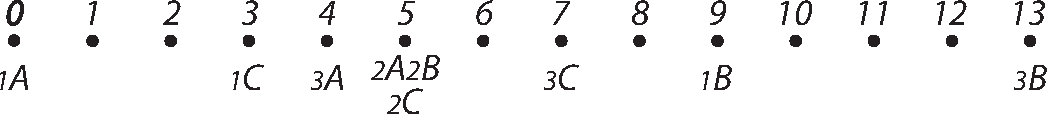
\includegraphics[width=0.73\textwidth]{%
gesamttex/edit_VIII,3/images/LH_37_05_104-105_d1_104r.pdf}}
\vspace{0.3em}
\centerline{%
\lbrack\textit{Fig.~1}\rbrack}
\newpage%
%
\pstart%
Ex transposita%
\protect\index{Sachverzeichnis}{aequatio transposita}
aeq. 13 fit
$5v + \overline{-1} \cdot x \overset{(15)}{=} \pleibvdash\, 4y + 8z \overset{(16)}{=} \text{duplo} \ 2c$
(per 2, 3, 4, 7),
seu progrediendi
%
\edtext{\lbrack velocitatem\rbrack}{%
\lemma{velocitas}\Bfootnote{%
\textit{L~ändert Hrsg.}}}
%
(\protect\vphantom)%
quae est summa velocitatum%
\protect\index{Sachverzeichnis}{summa velocitatum}
ejusdem corporis ante et post ictum,%
\protect\index{Sachverzeichnis}{velocitas ante ictum}%
\protect\index{Sachverzeichnis}{velocitas post ictum}
si sunt conspirantes;%
\protect\index{Sachverzeichnis}{velocitates conspirantes}
et differentia,%
\protect\index{Sachverzeichnis}{differentia velocitatum}
si contrariae%
\protect\index{Sachverzeichnis}{velocitates contrariae}%
\protect\vphantom()
esse aequalem duplae velocitati centri gravitatis%
\protect\index{Sachverzeichnis}{centrum gravitatis}%
\protect\index{Sachverzeichnis}{velocitas centri gravitatis dupla}
adeoque in ambobus corporibus esse eandem.
Seu quod eodem redit,
intervallum
(\protect\vphantom)%
\textit{{\scriptsize1}A{\scriptsize3}A}
vel
\textit{{\scriptsize1}B{\scriptsize3}B}%
\protect\vphantom()
inter loca%
\protect\index{Sachverzeichnis}{locus ab ictu remotus}
%
\edtext{ejusdem corporis}{%
\lemma{ejusdem}\Bfootnote{%
\hspace{-0,5mm}corporis
\textit{erg.~L}}}
%
ante et post ictum
eodem intervallo temporis%
\protect\index{Sachverzeichnis}{intervallum temporis}
ab ictu remota,
seu progressum corporis%
\protect\index{Sachverzeichnis}{progressus corporis}
toto tempore%
\protect\index{Sachverzeichnis}{tempus cujus medio factus est ictus}
cujus medio factus est ictus%
\protect\index{Sachverzeichnis}{ictus}
(\protect\vphantom)%
in eam partem
in quam revera toto hoc tempore progressum deprehenditur%
\protect\vphantom()
esse aequalem progressui centri gr.\ eodem tempore facto,%
\protect\index{Sachverzeichnis}{progressus centri gravitatis}
atque adeo in ambobus corporibus esse aequalem.
Unde et%
\lbrack,\rbrack\
%
\edtext{si velocitates corporum propriae%
\protect\index{Sachverzeichnis}{velocitas corpori propria}
dicantur eae
quae sunt ipsis reciproce proportionales,%
\protect\index{Sachverzeichnis}{velocitas corpori reciproce proportionalis}%
}{%
\lemma{si velocitates \lbrack...\rbrack\ proportionales}\Cfootnote{%
Siehe C.~\textsc{Wren}, \glqq Theory\grqq, \textit{PT} 1669, S.~867.\cite{01066}% concerning the same subject
}}
%
ita scilicet ut occurrerent sibi in centro gravitatis,%
\protect\index{Sachverzeichnis}{occursus in centro gravitatis}%
\protect\index{Sachverzeichnis}{centrum gravitatis}
%
\edtext{\lbrack dici\rbrack}{%
\lemma{dicit}\Bfootnote{%
\textit{L~ändert Hrsg.}}}
%
potest,
%
\edtext{%
quantum corpus tota velocitate ante ictum excedit velocitatem propriam,%
\protect\index{Sachverzeichnis}{velocitas corpori propria}
tantum idem post ictum tota velocitate deficit infra velocitatem propriam%
\protect\index{Sachverzeichnis}{velocitas corpori propria}
vel contra.
Differentia autem velocitatis totalis a propria%
\protect\index{Sachverzeichnis}{differentia velocitatis totalis a propria}%
\protect\index{Sachverzeichnis}{velocitas totalis}%
\protect\index{Sachverzeichnis}{velocitas corpori propria}
est velocitas communis,%
\protect\index{Sachverzeichnis}{velocitas communis}
ipsius scilicet centri gravitatis.%
\protect\index{Sachverzeichnis}{velocitas centri gravitatis}
Adeoque haec differentia non tantum in utroque tempore seu statu,%
\protect\index{Sachverzeichnis}{status}
sed etiam in utroque corpore eadem est.%
}{%
\lemma{\textit{Am Rand:}}\Afootnote{%
Velocitas propria corporis diversa
prout cum diversis confertur.\vspace{-2mm}}}
%
\pend%
%
\pstart%
Porro si aequ.~11 ducas in aeq.~15,
dextrum in dextrum,
sinistrum in sinistrum,
fit
\protect\rule[-3mm]{0mm}{8mm}$6a \cdot \overline{25v^2 - 1 \cdot x^2} \overset{(17)}{=} 3b \cdot \overline{64z^2 - 16y^2},$
seu differentiae quadratorum a velocitatibus%
\protect\index{Sachverzeichnis}{quadratum velocitatis}%
\protect\index{Sachverzeichnis}{differentia quadratorum velocitatum}
ejusdem corporis ante et post ictum,%
\protect\index{Sachverzeichnis}{ictus}
sunt corporibus reciproce proportionales.
Hinc et patet,
si unius corporis velocitas augetur ictu,%
\protect\index{Sachverzeichnis}{velocitas ictu aucta}
alterius velocitatem minui ictu.%
\protect\index{Sachverzeichnis}{velocitas ictu minuta}
Sublata est ambiguitas in hac aequatione, % ; %
\protect\index{Sachverzeichnis}{ambiguitas sublata in aequatione}
%\lbrack,\rbrack\
seu signum $\pleibdashv.$%
\protect\index{Sachverzeichnis}{signum ambiguum}
Ex transposita aequatione 17 fit%
\protect\index{Sachverzeichnis}{aequatio transposita}
$6a25v^2 + 3b16y^2 \overset{(18)}{=}
\edtext{[6]a1x^2}{\lemma{3\; \textit{L~ändert}}\Bfootnote{\hspace{-0,5mm}\textit{Hrsg.}}}
+ 3b64z^2.$
Hoc est,
summa potentiae est eadem ante et post ictum.%
\protect\index{Sachverzeichnis}{summa potentiae ante ictum}%
\protect\index{Sachverzeichnis}{summa potentiae post ictum}
\pend%
%
\pstart%
Ex his varia colligas,
ut ex aeq.~12
si ambo corpora ferantur ad easdem partes ante et post concursum,
servatur quantitatum motus summa,%
\protect\index{Sachverzeichnis}{summa quantitatum motus servata}%
\protect\index{Sachverzeichnis}{quantitas motus}
si in contrarias differentia;%
\protect\index{Sachverzeichnis}{differentia quantitatum motus servata}
si neutrum,
%
\edtext{tunc differentia quantitatum unius status
aequatur summae quantitatum alterius status.%
\protect\index{Sachverzeichnis}{status}%
\protect\index{Sachverzeichnis}{quantitas motus}%
}{%
\lemma{tunc}\Bfootnote{%
\textit{(1)}~differentia
\textbar~quantitatum \textit{erg.}~%
\textbar\ status ante vel post ictum aequatur summae post vel ante ictum.
\textit{(2)}~differentia quantitatum \lbrack...\rbrack\ alterius status.%
~\textit{L}}}
%
\pend%
\newpage
\pstart%
Corpus quod antecedit centrum gravitatis%
\protect\index{Sachverzeichnis}{corpus centrum gravitatis antecedens}%
\protect\index{Sachverzeichnis}{centrum gravitatis}
semper pergit ad easdem partes,%
\protect\index{Sachverzeichnis}{corpus pergens ad easdem partes}
quod contrait centro gravitatis%
\protect\index{Sachverzeichnis}{corpus centro gravitatis contraiens}%
\protect\index{Sachverzeichnis}{centrum gravitatis}
semper reflectitur,%
\protect\index{Sachverzeichnis}{corpus reflexum}
denique quod insequitur[,]
pone[,]
centrum gravitatis,%
\protect\index{Sachverzeichnis}{corpus centrum gravitatis insequens}
si plus quam duplo celerius fertur centro,%
\protect\index{Sachverzeichnis}{centrum gravitatis}
post concursum repercutitur%
\protect\index{Sachverzeichnis}{corpus repercussum}% , 
\lbrack;\rbrack\
sin minus pergit% , 
\lbrack;\rbrack\
si exacte duplo celerius quiescit.%
\protect\index{Sachverzeichnis}{corpus quiescens post concursum}
Cum omnia in easdem partes tendunt,%
\protect\index{Sachverzeichnis}{corpus in easdem partes tendens}
satis apparet
quod corpus antecedat%
\protect\index{Sachverzeichnis}{corpus centrum gravitatis antecedens}
aut sequatur centrum gravitatis%
\protect\index{Sachverzeichnis}{corpus centrum gravitatis sequens}%
\lbrack;\rbrack\
sed si corpora sibi occurrunt,%
\protect\index{Sachverzeichnis}{corpora sibi occurrentia}
tunc in easdem partes cum centro gravitatis it % ,
ipsumque persequitur illud corpus%
\protect\index{Sachverzeichnis}{corpus centrum gravitatis persequens}
cujus major est quantitas motus,%
\protect\index{Sachverzeichnis}{quantitas motus major}
contrait cujus minor,%
\protect\index{Sachverzeichnis}{corpus centro gravitatis contraiens}%
\protect\index{Sachverzeichnis}{quantitas motus minor}
si aequalis amborum,%
\protect\index{Sachverzeichnis}{quantitas motus aequalis}
centrum gravitatis quiescit.%
\protect\index{Sachverzeichnis}{centrum gravitatis}%
\protect\index{Sachverzeichnis}{corpus quiescens post concursum}
%
\lbrack104~v\textsuperscript{o}\rbrack\  %  %  %  %  Blatt 104v
%
\pend%
\vspace{0.1em}
\pstart%
\edtext{Vis ictus:%
\protect\index{Sachverzeichnis}{vis ictus}%
\protect\index{Sachverzeichnis}{ictus}
\textit{ab} in $\overline{a + b},$
vis tota:%
\protect\index{Sachverzeichnis}{vis tota}
$ab + cc$ in $\overline{a + b} = avv + byy.$
%
\edtext{Hinc vis ictus
qua corpora in se invicem in concursu agunt,%
\protect\index{Sachverzeichnis}{corpora concurrentia}%
\protect\index{Sachverzeichnis}{concursus corporum}
est ad vim reliquam%
\protect\index{Sachverzeichnis}{vis reliqua}%
}{%
\lemma{Hinc}\Bfootnote{%
\hspace{-0,5mm}vis ictus
\textit{(1)}~a vi
\textit{(2)}~ad vim
\textit{(3)}~qua corpora % in se invicem in concursu agunt, est ad 
\lbrack...\rbrack\ vim reliquam%
~\textit{L}}}
%
ut rectangulum sub velocitatibus propriis%
\protect\index{Sachverzeichnis}{velocitas corpori propria}%
\protect\index{Sachverzeichnis}{rectangulum sub velocitatibus propriis}
ad quadratum velocitatis communis.%
\protect\index{Sachverzeichnis}{quadratum velocitatis communis}%
\protect\index{Sachverzeichnis}{velocitas communis}%
}{%
\lemma{\textit{Am Rand hervorgehoben.}}\Afootnote{%
%Vis ictus \lbrack...\rbrack\ communis:
\newline%
}}
%
In corporibus%
\protect\index{Sachverzeichnis}{corpus molle}
%
\edlabel{37_05_104-105_1a}%
mollibus vel imperfecte Elasticis%
\protect\index{Sachverzeichnis}{corpus imperfecte elasticum}%
\protect\index{Sachverzeichnis}{corpus elasticum}
perditur vis ictus.%
\protect\index{Sachverzeichnis}{vis ictus perdita}%
\protect\index{Sachverzeichnis}{ictus}%
\edtext{}{%
{\xxref{37_05_104-105_1a}{37_05_104-105_1b}}%
{\lemma{mollibus}\Bfootnote{%
\textit{(1)}~perditur vis ictus,
\textit{(2)}~vel imperfecte Elasticis perditur vis ictus.%
~\textit{L}}}}
%
\pend%
\vspace{0.5em}%
%
\pstart%
\noindent%
\lbrack\textit{Nachfolgend kleingedruckter Text in L gestrichen:}\rbrack\
\pend%
\vspace{0.5em}%
%
\footnotesize%
\pstart%
Porro
%
\edtext{per aeq.~5,}{%
\lemma{per}\Bfootnote{%
\textit{(1)}~(5)
\textit{(2)}~aeq.~5,%
~\textit{L}}}
%
si ex corporis tota velocitate ante ictum 5\textit{v}%
\protect\index{Sachverzeichnis}{velocitas ante ictum}
detrahatur duplum velocitatis propriae seu $(2)3b,$%
\protect\index{Sachverzeichnis}{velocitas corpori propria}
residua erit tota ejus velocitas post ictum,%
\protect\index{Sachverzeichnis}{velocitas post ictum}
seu $\overline{-1} \!\cdot\! x.$
\pend%
\vspace{0.6em}%
%
\normalsize%
\pstart%
Porro%
\edlabel{37_05_104-105_1b}
$\overline{-1} \!\cdot\! x = 2c - 3b$
et
$2c = 6a \;\pleibvdash\, 4y.$
Ergo si corpus \textit{B} sit quiescens,
seu
$y = 0,$
fiet
$\overline{-1} \!\cdot\! x = 6a - 3b.$
Seu in casu
quo corpus \textit{A} motum%
\protect\index{Sachverzeichnis}{corpus motum}
impingit in \textit{B} quiescens,%
\protect\index{Sachverzeichnis}{corpus quiescens ante ictum}
erit
$\overline{-1} \!\cdot\! x$
velocitas ipsius \textit{A} post ictum%
\protect\index{Sachverzeichnis}{velocitas post ictum}
aequalis velocitati propriae%
\protect\index{Sachverzeichnis}{velocitas corpori propria}
%
\edtext{ipsius \textit{B} detracta}{%
\lemma{ipsius}\Bfootnote{%
\textit{(1)}~\textit{A} detracta
\textit{(2)}~\textit{B} detracta%
~\textit{L}}}
%
velocitate propria%
\protect\index{Sachverzeichnis}{velocitas corpori propria}
%
\edtext{ipsius \textit{A}.
Rursus}{%
\lemma{ipsius}\Bfootnote{%
\hspace{-0,5mm}\textit{A}.
\textit{(1)}~Ergo
\textit{(2)}~Rursus%
~\textit{L}}}
%
per aeq.~1,
quando $y = 0,$
fit
$5v = 3b + 6a.$
Ergo
$5v : \overline{-1} \!\cdot\! x \,\squaredots\, 6a + 3b : 6a - 3b.$
Seu
%
\edtext{%
\edlabel{LH_37_05_104v_scwitch-1}%
\textls{quando corpus \textit{A} motum%
\protect\index{Sachverzeichnis}{corpus motum}
impingit in corpus \textit{B} quiescens,%
\protect\index{Sachverzeichnis}{corpus quiescens ante ictum}
erit celeritas corporis \textit{A} ante ictum,%
\protect\index{Sachverzeichnis}{celeritas ante ictum}
ad celeritatem ejusdem post ictum,%
\protect\index{Sachverzeichnis}{celeritas post ictum}
ut summa corporum%
\protect\index{Sachverzeichnis}{summa corporum}
ad eorum differentiam.%
\protect\index{Sachverzeichnis}{differentia corporum}%
\protect\index{Sachverzeichnis}{ictus}%
}%
\edlabel{LH_37_05_104v_scwitch-2}%
}{%
\lemma{\textit{Quer am Rand, gestr. und abbrechend:}}\Afootnote{%
{\footnotesize%
Itaque in medio}\vspace{-2mm}}}
\pend
\count\Bfootins=1000%
\count\Afootins=1200%
\count\Cfootins=1000
\pstart%
Unde sequitur%
\edlabel{LH_37_05_104v_resistinmedio-1}
%
\edtext{\lbrack corpore\rbrack}{%
\lemma{corpora}\Bfootnote{%
\textit{L~ändert Hrsg.}}}
%
\textit{A} in medium aliquod impingente,%
\protect\index{Sachverzeichnis}{corpus impingens in medium}%
\protect\index{Sachverzeichnis}{medium}
nempe in partes ejus
quae sint ut \textit{B}
%
\edtext{quiescentes,%
\protect\index{Sachverzeichnis}{partes medii quiescentes}
semper in eadem ratione,}{%
\lemma{quiescentes,}\Bfootnote{%
\textit{(1)}~\textbar~semper easdem, \textit{streicht Hrsg.}~\textbar\
\textit{(2)}~semper in eadem ratione,%
~\textit{L}}}
%
nempe $A + B$ ad $A - B$
diminui velocitatem ipsius \textit{A},%
\protect\index{Sachverzeichnis}{velocitas diminuta}
atque adeo diminutiones velocitatum
esse velocitatibus proportionales.%
\protect\index{Sachverzeichnis}{diminutio velocitatis velocitati proportionalis}
%
\edtext{Seu spatiis positis aequalibus
decrementa velocitatum
esse velocitatibus proportionalia%
\protect\index{Sachverzeichnis}{decrementum velocitatis velocitati proportionale}
et proinde temporibus aequalibus
esse ut velocitatum quadrata.
Nam $ds = v\,dt.$
Vide quid dicendum,
cum medium in corpus incurrit.%
\edlabel{LH_37_05_104v_resistinmedio-2}%
\protect\index{Sachverzeichnis}{medium incurrens in corpus}%
}{%
\lemma{Seu}\Bfootnote{%
\hspace{-0,5mm}spatiis
\lbrack...\rbrack\ Nam $ds = vdt.$
\textit{(1)}~Cum autem peri
\textit{(2)}~Vide quid % dicendum, ...
\lbrack...\rbrack\ corpus incurrit.
\textit{erg.~L}}}
%
\pend
%
\pstart%
Rursus
quia per aeqq.~4 et 8 habemus:
$\overline{-1} \!\cdot\! x = 5v - (2)3b$
et
$8z = \;\pleibvdash\, 4y + (2)6a,$
hinc
si corpus \textit{A} et corpus \textit{B}
tendant in easdem%
\protect\index{Sachverzeichnis}{corpus in easdem partes tendens}
%
\edtext{partes,
fit
$z = y + (2)a.$
Itaque
si temporis exiguo quovis aequali intervallo%
\protect\index{Sachverzeichnis}{intervallum temporis exiguum}%
}{%
\lemma{partes,}\Bfootnote{%
\textit{(1)}~fit $8z = +\, y + (2)6a$
\textit{(2)}~fit $z = y + (2)a.$
\textit{(a)}~Itaque si quovis temporis
\textbar~exiguo \textit{erg.}~%
\textbar\ intervallo
\textit{(b)}~Itaque si % temporis exiguo quovis 
\lbrack...\rbrack\ aequali intervallo%
~\textit{L}}}
%
corpus \textit{B} novum impetum recipere%
\protect\index{Sachverzeichnis}{impetus novus receptus}
%
\edtext{intelligatur
a corpusculo impacto%
\protect\index{Sachverzeichnis}{corpusculum impactum}
quale est \textit{A},%
}{%
\lemma{intelligatur}\Bfootnote{%
\textit{(1)}~a corpore quale est \textit{A}
\textit{(2)}~a corpusculo % impacto quale 
\lbrack...\rbrack\ est \textit{A},%
~\textit{L}}}
%
\pend%
\vspace{0.5em}%
%
\pstart%
\noindent%
\lbrack\textit{Nachfolgend kleingedruckter Text in L gestrichen:}\rbrack\
\pend%
\vspace{0.5em}%
%
\footnotesize%
\pstart%
\noindent%
eadem semper manente velocitate \textit{y} ipsius \textit{A},
nempe \textit{y};
ponatur
%
\edtext{autem $2(a),$}{%
\lemma{autem}\Bfootnote{%
\textit{(1)}~2\textit{A},
\textit{(2)}~$2(a),$%
~\textit{L}}}
%
hoc est velocitas propria ipsius \textit{B},%
\protect\index{Sachverzeichnis}{velocitas corpori propria}
manere semper eadem
%
\edtext{circiter;
atque adeo}{%
\lemma{circiter;}\Bfootnote{%
\textit{(1)}~seu
\textit{(2)}~atque adeo%
~\textit{L}}}
%
intervallum inter \textit{A} et \textit{B} % ,
quod eo tempore absolvitur%
\protect\index{Sachverzeichnis}{intervallum temporis}
(\protect\vphantom)%
nam quia \textit{a} velocitas propria eadem%
\protect\index{Sachverzeichnis}{velocitas corpori propria}
%
\edtext{manet,
et corpora \textit{A} et \textit{B} semper aequalia manent,
etiam}{%
\lemma{manet,}\Bfootnote{%
\textit{(1)}~etiam
\textit{(2)}~et corpora % \textit{A} et \textit{B} semper aequalia 
\lbrack...\rbrack\ manent, etiam%
~\textit{L}}}
%
corporum intervallum semper aequale%
\protect\index{Sachverzeichnis}{intervallum corporum}
%
\edtext{manet,
hujus enim}{%
\lemma{manet,}\Bfootnote{%
\textit{(1)}~nempe qu
\textit{(2)}~hujus enim%
~\textit{L}}}
%
in ratione certa portio est \textit{a}%
\protect\vphantom()
quoniam ipsius \textit{B} motus,%
\protect\index{Sachverzeichnis}{motus exiguus}
qui differentiam facere possit,
exiguus est respectu motus celerrimi%
\protect\index{Sachverzeichnis}{motus celerrimus}
ipsius \textit{A} % ,
in ipsum impingentis,%
\protect\index{Sachverzeichnis}{motus corporis impingentis}
atque adeo progressus%
\protect\index{Sachverzeichnis}{progressus corporis impingentis}
%
\edtext{ipsius \textit{B}% , 
}{%
\lemma{ipsius}\Bfootnote{%
\textit{(1)}~\textit{A}
\textit{(2)}~\textit{B}%
~\textit{L}}}
%
durante motu ipsius \textit{A}
in exiguo illo tempore%
\protect\index{Sachverzeichnis}{tempus exiguum}
in considerationem non venit,%
\protect\index{Sachverzeichnis}{consideratio}
hinc
posita $(2)a$ semper aequali
\edlabel{LH_37_05_104v_udyf-1}%
corpus
{\normalsize{\lbrack\textit{Text bricht ab.}\rbrack}}
%
\edtext{}{%
{\xxref{LH_37_05_104v_udyf-1}{LH_37_05_104v_udyf-2}}%
{\lemma{corpus}\Bfootnote{%
\textit{(1)}~est autem \textit{y} semper
\textit{(2)}~itaque
\textit{(c)}~tunc \textit{y} semper%
~\textit{L}}}}%
%
\pend%
\vspace{0.5em}%
%
\footnotesize%
\pstart%
\noindent%
tunc \textit{y} semper%
\edlabel{LH_37_05_104v_udyf-2}
manente,
tantum examinandum
quomodo crescat $(2)a,$
seu quomodo
%
\edtext{crescat \textit{a}.
Crescit autem \textit{a},
distantia corporis \textit{B} a centro gravitatis communi,%
\protect\index{Sachverzeichnis}{distantia a centro gravitatis}
in ea}{%
\lemma{crescat \textit{a}.}\Bfootnote{%
\textit{(1)}~Sit ergo corpus
\textit{(2)}~Crescit autem \textit{a},
\textit{(a)}~in ea
\textit{(b)}~distantia corporis % \textit{B} a centro gravitatis communi, 
\lbrack...\rbrack\ in ea%
~\textit{L}}}
%
ratione,
in qua crescunt intervalla corporum%
\protect\index{Sachverzeichnis}{intervallum corporum}
{\normalsize{\lbrack\textit{Text bricht ab.}\rbrack}}%
%
\pend%
\vspace{0.5em}%
%
\footnotesize%
\pstart%
\noindent%
tunc posito intervallum%
\protect\index{Sachverzeichnis}{intervallum corporum}
inter corpora \textit{A} et \textit{B} % , 
initio tempusculi esse semper aequale,%
\protect\index{Sachverzeichnis}{tempusculum}
adeoque et \textit{a} distantiam ipsius \textit{B} a centro gravitatis communi,%
\protect\index{Sachverzeichnis}{centrum gravitatis commune}
%
\edtext{\lbrack quod\rbrack}{%
\lemma{quae}\Bfootnote{%
\textit{L~ändert Hrsg.}}}
%
distantiam in ratione corporum secat,%
\protect\index{Sachverzeichnis}{distantia corporum}%
\protect\index{Sachverzeichnis}{distantia secta in ratione corporum}
esse semper aequalem,
atque adeo et duplum ejus, $2a,$
manifestum est variari \textit{y},
seu dum
{\normalsize{\lbrack\textit{Text bricht ab.}\rbrack}}%
\pend%
\vspace{0.5em}%
%
\normalsize%
\pstart%
\noindent%
tunc posito \textit{y} velocitatem esse semper aequalem,%
\protect\index{Sachverzeichnis}{velocitas corporis impingentis}
qua corpus \textit{A} impingit in corpus \textit{B},
necesse est distantiam
ex qua
%
\edtext{corpus \textit{A} dato tempore venit}{%
\lemma{corpus \textit{A}}\Bfootnote{%
\textit{(1)}~exiguo illo tempusculo ve%
\protect\index{Sachverzeichnis}{tempusculum}
\textit{(2)}~assumto
\textit{(3)}~dato tempore venit%
~\textit{L}}}
%
esse minorem,
quia alioqui%
\lbrack,\rbrack\
cum \textit{B} interim
%
\edtext{celerius progrediatur,}{%
\lemma{celerius}\Bfootnote{%
\textit{(1)}~prosequat
\textit{(2)}~progrediatur,%
~\textit{L}}}
%
%
\edtext{corpus \textit{A} ipsum}{%
\lemma{corpus \textit{A}}\Bfootnote{\hspace{-0,5mm}%
\textbar~alias \textit{gestr.}~%
\textbar\ ipsum%
~\textit{L}}}
%
eadem celeritate hoc tempore assequi non posset.%
\protect\index{Sachverzeichnis}{corpus assequens}
Itaque et \textit{a} est major,
quae est portio hujus distantiae in
%
\edtext{ratione corporis \textit{A},
ad}{%
\lemma{ratione}\Bfootnote{%
\textit{(1)}~\textit{a} ad
\textit{(2)}~corporis \textit{A}, ad%
~\textit{L}}}
%
corporum summam%
\protect\index{Sachverzeichnis}{summa corporum}
%
%\edlabel{37_05_104-105_2a}%
$A + B.$%
\pend%
\newpage
\pstart%
\noindent%
\lbrack\textit{Nachfolgend kleingedruckter Text in L gestrichen:}\rbrack\
\pend%
\vspace{0.5em}%
%
\footnotesize%
\pstart%
\noindent%
Est autem tanto major distantia,%
\protect\index{Sachverzeichnis}{distantia corporum sese insequentium}
quanta est
%
\edtext{prior \textit{z}.
Ergo
$\displaystyle \langle m \cdot \overline{lz}\rangle = z.$%
}{%
\lemma{prior.}\Bfootnote{%
\textit{(1)}~$y + z$
\textit{(2)}~\textit{z}
\textbar~seu distantia corporum sese insequentium, quae est initio motus \textit{erg. u. gestr.}~%
\textbar\ Ergo
\textit{(a)}~$\displaystyle z \, =$
\textit{(b)}~$\displaystyle \langle m \cdot \overline{lz}\rangle = z.$%
~\textit{L}}}
%
Seu \textit{l}, $1 + l,$ $\overline{1 + 1 + l},$ $1 + 1 + 1 + l.$
Ergo incrementa sunt progressionis Arithmeticae,%
\protect\index{Sachverzeichnis}{incrementum velocitatis}%
\protect\index{Sachverzeichnis}{progressio arithmetica}
seu aequalibus temporibus aequaliter crescunt.%
\protect\index{Sachverzeichnis}{tempus aequale}
% {\normalsize{\lbrack\textit{Text bricht ab.}\rbrack}}
%
{\normalsize{\lbrack105~r\textsuperscript{o}\rbrack}}  % % % Blatt 105r
%
\pend%
\vspace{0.5em}%
%
\normalsize%
\pstart%
\noindent%
Jam
%\edlabel{37_05_104-105_2b}
%
distantia corporum $A + B$ sese insequentium,%
\protect\index{Sachverzeichnis}{distantia corporum sese insequentium}
exprimitur per differentiam celeritatum,%
\protect\index{Sachverzeichnis}{differentia celeritatum}
posito celeritates exprimi per spatia%
\protect\index{Sachverzeichnis}{celeritas expressa per spatium}
quae dato tempore absolvunt,%
\protect\index{Sachverzeichnis}{spatium absolutum tempore dato}
seu per $x - y,$
et
$a = A \cdot \overline{x - y} : \overline{A + B}.$
Ergo
$z = Ay + By + Ax - Ay,\, : \overline{A + B}.$
Seu
$z = Ax + By,\, :
%
%\edlabel{37_05_104-105_3a}%
A + B.$%
\pend%
\vspace{1.0em}%
%
\pstart%
\noindent%
\lbrack\textit{Nachfolgend kleingedruckter Text in L gestrichen:}\rbrack\
\pend%
\vspace{0.5em}%
%
\footnotesize%
\pstart%
\noindent%
Itaque habemus praeclarum theorema,%
\protect\index{Sachverzeichnis}{theorema praeclarum}
quod in medio aequabiliter impellente et ubique uniformi,%
\protect\index{Sachverzeichnis}{medium aequabiliter impellens}%
\protect\index{Sachverzeichnis}{medium ubique uniforme}
incrementa velocitatum sint temporibus proportionalia%
\protect\index{Sachverzeichnis}{incrementum velocitatis proportionale tempori}
%
\edtext{uti in gravium acceleratione%
\protect\index{Sachverzeichnis}{acceleratio gravium}
posuit Galilaeus.%
\protect\index{Namensregister}{\textso{Galilei} (Galilaeus, Galileus), Galileo 1564\textendash1642}%
}{%
\lemma{uti \lbrack...\rbrack\ Galilaeus}\Cfootnote{%
Vgl. G.~\textsc{Galilei}, \textit{Discorsi}, dialogo III, theorema~1, prop.~1
(Leiden 1638, S.~169\textendash171;\cite{00050}
\textit{GO} VIII, S.~208\,f.).\cite{00048}%
}}
%
Sed hinc sequitur
ipsas \textit{z} esse progressionis Geometricae.%
\protect\index{Sachverzeichnis}{progressio Geometrica}
Sit
%
\edtext{enim $Z%
}{%
\lemma{enim}\Bfootnote{%
\textit{(1)}~\textit{z}
\textit{(2)}~\textit{Z}%
~\textit{L}}}
%
= l,$
%
\edtext{fiet $\textit{(}Z\textit{)}%
}{%
\lemma{fiet}\Bfootnote{%
\textit{(1)}~\textit{Z}
\textit{(2)}~\textit{(Z)}%
~\textit{L}}}
%
= Z + m,$
$Z = l + al
%
\edtext{= l \cdot \overline{1 + a},$}{%
\lemma{$=$}\Bfootnote{%
\hspace{-0,5mm}$l \cdot \overline{1 + a}$
\textit{erg.~L}}}
%
\edtext{et $\textit{((}Z\textit{))}%
}{%
\lemma{et}\Bfootnote{%
\textit{(1)}~\textit{z}
\textit{(2)}~\textit{((Z))}%
~\textit{L}}}
%
= \textit{(}Z\textit{)} + m\textit{(}Z\textit{)}$
seu
$l + ml + ml +
%
\edtext{m^2l,\, = l \cdot \protect\fbox{2}\;\overline{1 + m},$%
}{%
\lemma{$m^2l,$}\Bfootnote{%
\textit{(1)}~seu
\textit{(2)}~$=$
\textit{(a)}~$l + 1,$
\textit{(b)}~$l \cdot \protect\fbox{2}\;\overline{1 + m},$%
~\textit{L}}}
%
et ita
%
\edtext{porro.
Itaque}{%
\lemma{porro.}\Bfootnote{%
\textit{(1)}~Sunt
\textit{(2)}~Itaque%
~\textit{L}}}
%
si in medio
%
\edtext{aliquo
uniformiter disseminata aequalia corpuscula%
\protect\index{Sachverzeichnis}{corpuscula uniformiter in medio disseminata}%
\protect\index{Sachverzeichnis}{corpuscula aequali celeritate impingentia}
aequalibus temporum intervallis%
\protect\index{Sachverzeichnis}{intervallum temporis aequale}
in corpus aliquod
aequali celeritate impingere%
\protect\index{Sachverzeichnis}{celeritas aequalis}% , 
}{%
\lemma{aliquo}\Bfootnote{%
\textit{(1)}~in quo di
\textit{(2)}~aequabiliter
\textit{(3)}~uniformiter disseminata
\textit{(a)}~corpora
\textit{(b)}~aequalia corpuscula
\textit{(aa)}~aequalibus temporibus aequali celeritate in
\textit{(bb)}~aequalibus temporum intervallis in
\textbar~in \textit{streicht Hrsg.}~%
\textbar\ corpus aliquod
\textbar~aequali celeritate \textit{erg.}~%
\textbar\ impingere%
~\textit{L}}}
%
idque in easdem semper partes propellere intelligantur,
incrementa velocitatum%
\protect\index{Sachverzeichnis}{incrementum velocitatis corporis impulsi}
%
\edtext{impulsi corporis%
\protect\index{Sachverzeichnis}{corpus impulsum}%
}{%
\lemma{impulsi}\Bfootnote{%
\hspace{-0,5mm}corporis
\textit{erg.~L}}}
%
erunt progressionis Geometricae.%
\protect\index{Sachverzeichnis}{progressio geometrica}
Supponitur
%
\edtext{autem corpusculum}{%
\lemma{autem}\Bfootnote{%
\textit{(1)}~corpus
\textit{(2)}~corpusculum%
~\textit{L}}}
%
incurrens%
\protect\index{Sachverzeichnis}{corpusculum incurrens}
eadem semper velocitate et linea venire
{\normalsize{\lbrack\textit{Text bricht ab.}\rbrack}}
%
\pend%
\normalsize%
\vspace{0.5em}
\pstart%
\noindent%
Cum
%\edlabel{37_05_104-105_3b}
%
ergo incrementum velocitatis%
\protect\index{Sachverzeichnis}{incrementum velocitatis corporis impulsi}
seu excessus super \textit{y} velocitatem priorem%
\protect\index{Sachverzeichnis}{excessus super velocitatem priorem}%
\protect\index{Sachverzeichnis}{velocitas prior}
sit
%
\edtext{bis \textit{a},
utique
is excessus erit bis
$A \cdot\; \overline{x-y} : \overline{A + B}$
seu
$Ax : \overline{A + B}$
minus:
$Ay : \overline{A + B}.$
Jam}{%
\lemma{bis}\Bfootnote{%
\hspace{-0,5mm}\textit{a}
\textit{(1)}~seu bis \textit{A}
\textit{(2)}~, utique is % excessus erit bis
\lbrack...\rbrack\
$A \cdot\; \overline{x-y} : \overline{A + B}$
\textit{(a)}~. Jam cum
\textit{(b)}~seu $Ax : \overline{A + B}$ minus: $Ay : \overline{A + B}.$ Jam%
~\textit{L}}}
%
\makebox[1.0\textwidth][s]{$Ax : \overline{A + B}$
est semper eadem quantitas%
\lbrack,\rbrack\
et
$Ay : \overline{A + B}$
variatur proportione prioris}
\pend
\vspace{1.5em}
\centerline{%
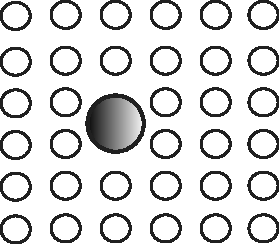
\includegraphics[width=0.20\textwidth]{%
gesamttex/edit_VIII,3/images/LH_37_05_104-105_d2_105r.pdf}}
\vspace{0.5em}
\centerline{%
\lbrack\textit{Fig.~2}\rbrack}
\newpage
\pstart
\noindent celeritatis.%
\protect\index{Sachverzeichnis}{celeritas prior}
%
\edtext{Itaque crementa}{%
\lemma{Itaque}\Bfootnote{%
\textit{(1)}~incrementa
\textit{(2)}~crementa%
~\textit{L}}}
%
seu differentiae velocitatum
a medio uniformiter impellente%
\protect\index{Sachverzeichnis}{crementum velocitatis a medio impellente}%
\protect\index{Sachverzeichnis}{differentia velocitatis a medio impellente}%
\protect\index{Sachverzeichnis}{medium uniformiter impellens}
%
\edtext{componuntur ex duobus,}{%
\lemma{componuntur}\Bfootnote{%
\hspace{-0,5mm}ex
\textit{(1)}~duabus,
\textit{(2)}~duobus,%
~\textit{L}}}
%
nempe ex incremento semper aequali%
\protect\index{Sachverzeichnis}{incrementum velocitatis aequale}
et ex decremento semper velocitatibus jam quaesitis proportionali,%
\protect\index{Sachverzeichnis}{decrementum velocitatis velocitati proportionale}%
\protect\index{Sachverzeichnis}{velocitas quaesita}
seu ex incremento Arithmetico%
\protect\index{Sachverzeichnis}{incrementum arithmeticum}
et decremento Geometrico.%
\protect\index{Sachverzeichnis}{decrementum geometricum}
%
\edlabel{LH_37_05_105r_aliunde-1}%
Et cum aliunde
%
%\edtext{aliunde}{%
%\lemma{aliunde}\Cfootnote{%
%Mit dem aus dem Widerstand des Mediums entstehenden \textit{detrimentum motus} hatte sich Leibniz bereits in Paris auseinandergesetzt und hierbei zwei Formen des Wiederstands unterschieden: eine nicht von der Geschwinbdigkeit des Körpers abhängige \textit{resistentia absoluta} (\textit{resistence absolue}) und eine mit der Geschwindigkeit wächsende \textit{resistentia respectiva} (\textit{resistence respective}).
%In beiden Fällen soll das \textit{detrimentum motus} nach geometrischer Progression wachsen.
%Siehe \textit{LSB} VIII,~2 N.~34\textsubscript{4}; N.~35; N.~36\textsubscript{1}; N.~36\textsubscript{2}.\cite{01368}\cite{01369}\cite{01370}\cite{01371}
%Ähnliche Ansichten wird Leibniz noch etwas später im \textit{Schediasma de resistentia medii et motu projectorum in medio resistente} vertreten (\textit{AE}, Januar 1689, S.~38\textendash47; \textit{LMG} VI, S.~135\textendash144).\cite{01024}}}
%
decrementa motus ex Medio resistente%
\protect\index{Sachverzeichnis}{decrementum motus e medio resistente}%
\protect\index{Sachverzeichnis}{medium resistens}
sint etiam velocitatibus proportionalia,%
\protect\index{Sachverzeichnis}{decrementum motus velocitati proportionale}%
\protect\index{Sachverzeichnis}{decrementum motus geometricum}
seu Geometrica,%
\edlabel{LH_37_05_105r_aliunde-2}
hinc in universum dici potest%
\lbrack:\rbrack\
si medium partim impellat,%
\protect\index{Sachverzeichnis}{medium impellens}
partim resistat,%
\protect\index{Sachverzeichnis}{medium resistens}%
\protect\index{Sachverzeichnis}{medium partim impellens partim resistens}
ut fit in gravium descensu,%
\protect\index{Sachverzeichnis}{descensus gravium}
incrementa velocitatis%
\protect\index{Sachverzeichnis}{incrementum velocitatis uniforme}
uniformia % , %
cum decrementis geometrice proportionalibus%
\protect\index{Sachverzeichnis}{decrementum velocitatis geometrice proportionale}
%
%\edlabel{37_05_104-105_4a}%
componi.%
%
%
\pend%
\vspace{1.0em}%
%
\pstart%
\noindent%
\lbrack\textit{Nachfolgend kleingedruckter Text in L gestrichen:}\rbrack\
\pend%
\vspace{0.5em}%
%
\footnotesize%
\pstart%
\noindent%
%
Quod si ipsum \textit{A} impellens tam parvum sit%
\protect\index{Sachverzeichnis}{corpusculum impellens}
ut prope nullam habeat rationem ad \textit{B},
%
\edtext{tunc $Ay : A + B$ haberi potest}{%
\lemma{tunc}\Bfootnote{%
\textit{(1)}~fit
\textit{(2)}~$Ay:A+B$ haberi potest%
~\textit{L}}}
%
pro nihilo,%
\protect\index{Sachverzeichnis}{nihilum}
%
\edtext{et pro vero haberi potest% , %
}{%
\lemma{et}\Bfootnote{%
\textit{(1)}~verum manet
\textit{(2)}~pro vero haberi potest% , %
~\textit{L}}}
%
\edtext{assumtum\edtext{ Galilaei,%
\protect\index{Namensregister}{\textso{Galilei} (Galilaeus, Galileus), Galileo 1564\textendash1642}%
\protect\index{Sachverzeichnis}{assumtum Galilaei}%
}{\lemma{assumtum Galilaei}\Cfootnote{%
%Vgl. \textsc{Galilei}, 
%\textit{Discorsi}, dialogo III, theorema 1, prop.~1
%(S.~169\textendash171; \textit{GO} VIII, S.~208\,f.).%
a.a.O.%
\cite{00048}\cite{00050}%
}}
%
idque verum est % , 
quamdiu loquimur
%
de aethere impellente%
\protect\index{Sachverzeichnis}{aether impellens}
qui est subtilissimus%
\protect\index{Sachverzeichnis}{aether subtilissimus}%
\lbrack,\rbrack\
neglecto aere resistente%
\protect\index{Sachverzeichnis}{aer resistens}
qui est satis crassus.%
\protect\index{Sachverzeichnis}{aer satis crassus}
Haec autem intelligenda sunt,
si celeritas \textit{x} corpusculi \textit{A} (impellentis)%
\protect\index{Sachverzeichnis}{celeritas corpusculi impellentis}%
\protect\index{Sachverzeichnis}{corpusculum impellens}
satis sit notabilis,%
\protect\index{Sachverzeichnis}{celeritas satis notabilis}%
}{%
\lemma{Galilaei}\Bfootnote{%
\textit{(1)}~. Verumtamen pro certo habendum est, non posse impune negligi quando celeri
\textit{(2)}~, idque verum est, quamdiu
\textbar~quamdiu \textit{streicht Hrsg.}~%
\textbar\ loquimur de aethere impellente
\textit{(a)}~, non quam
\textit{(b)}~qui est % subtilissimus neglecto aere resistente, qui est 
\lbrack...\rbrack\ satis crassus.
\textit{(aa)}~Et quidem quamdiu
\textit{(aaa)}~\textit{x}
\textit{(bbb)}~celeritatis \textit{x} corpusculi
\textit{(bb)}~Haec autem % intelligenda sunt, si celeritas \textit{x} corpusculi \textit{A} (impellentis) satis 
\lbrack...\rbrack\ sit notabilis,%
~\textit{L}}}
%
respectu celeritatis \textit{y} a corpore impulso acquisitae,%
\protect\index{Sachverzeichnis}{celeritas quaesita a corpore impulso}%
\protect\index{Sachverzeichnis}{corpus impulsum}
alioqui enim
si et \textit{x} quasi infinite parva esset,%
\protect\index{Sachverzeichnis}{celeritas infinite parva}
tunc
{\normalsize{\lbrack\textit{Text bricht ab.}\rbrack}}
%
\pend%
\vspace{1.0em}%
%
\normalsize%
\pstart%
\noindent%
Itaque
%\edlabel{37_05_104-105_4b}
%
ut locum habeat
%
\edtext{Hypothesis Galilaei%
\protect\index{Namensregister}{\textso{Galilei} (Galilaeus, Galileus), Galileo 1564\textendash1642}%
\protect\index{Sachverzeichnis}{hypothesis Galilaei}%
}{%
\lemma{Hypothesis Galilaei}\Cfootnote{%
%Vgl. \textsc{Galilei}, \textit{Discorsi}, 3.~Tag, theorema I, prop.~1
%(S.~????; \textit{GO} VIII, S.~208\,f.).%
a.a.O.%
\cite{00048}\cite{00050}%
}}
%
necesse est % ,
\textit{x}
%
\edtext{celeritatem corpusculi \textit{A}%
\protect\index{Sachverzeichnis}{celeritas corpusculi impellentis}
impellentis corpus \textit{B}%
\protect\index{Sachverzeichnis}{corpus impulsum a medio}
incomparabiliter}{%
\lemma{celeritatem}\Bfootnote{%
\textit{(1)}~corporis \textit{A} incompa
\textit{(2)}~corpusculi \textit{A} impellentis
\textbar~corpus \textit{B} \textit{erg.}~%
\textbar\ incomparabiliter%
~\textit{L}}}
%
majorem esse
%
\edtext{quam \textit{y} impetum a corpore}{%
\lemma{quam}\Bfootnote{%
\textit{(1)}~celeritatem a cor
\textit{(2)}~\textit{y} impetum a corpore%
~\textit{L}}}
%
\textit{B} jam acquisitum,%
\protect\index{Sachverzeichnis}{impetus acquisitus a corpore impulso}
ita enim decrementum proportionale%
\protect\index{Sachverzeichnis}{decrementum velocitatis velocitati proportionale}
$Ay : \overline{A + B}$
negligi potest
prae incremento aequabili%
\protect\index{Sachverzeichnis}{incrementum velocitatis aequabile}
$Ax : \overline{A + B}.$
\pend%
%
\pstart%
Itaque
quando corpora magnam velocitatem acquisivere%
\protect\index{Sachverzeichnis}{velocitas acquisita ab impetu impresso}
ab impresso impetu,%
\protect\index{Sachverzeichnis}{impetus impressus a medio}
notabile fit
%
\edtext{decrementum.%
\protect\index{Sachverzeichnis}{decrementum velocitatis notabile}
Sed hoc}{%
\lemma{decrementum}\Bfootnote{%
\textit{(1)}~, non tantum et propo
\textit{(2)}~. Sed hoc%
~\textit{L}}}
%
decrementum cum resistentia aeris%
\protect\index{Sachverzeichnis}{resistentia aeris}
in unum confundi tuto potest,
quamdiu in eodem semper medio,
nempe aere%
\protect\index{Sachverzeichnis}{aer medius}
motus computatur.%
\protect\index{Sachverzeichnis}{motus computatus in medio}
Pluribus autem mediis adhibitis%
\protect\index{Sachverzeichnis}{medium adhibitum}
putem experimentis determinari posse%
\protect\index{Sachverzeichnis}{experimentum pluribus mediis adhibitis}
quanta sit celeritas \textit{x},
et quanta magnitudo \textit{A}.
%
\lbrack105~v\textsuperscript{o}\rbrack\ % Blatt 105v
%
\pend%
\newpage%
\centerline{%
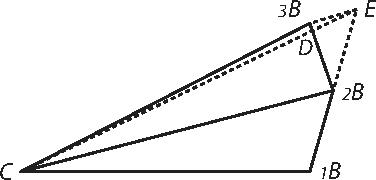
\includegraphics[width=0.42\textwidth]{%
gesamttex/edit_VIII,3/images/LH_37_05_104-105_d3_105v.pdf}}
\vspace{0.5em}
\centerline{%
\lbrack\textit{Fig.~3}\rbrack}%
\label{LH_37_05_105v_Fig.3}%
%\newpage%
\vspace{1.3em}
%
%
\count\Bfootins=1000%
\count\Afootins=1200%
\count\Cfootins=1000 
\pstart%
%%%% GETRIXT:
\edtext{}{\lemma{\hspace{1,6mm}\lbrack\textit{Fig.~3}\rbrack}\killnumber\Cfootnote{%
Vgl. das Diagramm a.a.O, S.~37.
}}%
Porro%
\edlabel{LH_37_05_105v_PhNPM_Stelle-1}
%
\edtext{observavit
%
\edtext{Keplerus%
\protect\index{Namensregister}{\textso{Kepler} (Keplerus), Johannes 1571\textendash1630}
areas Ellipseos%
\protect\index{Sachverzeichnis}{area ellipseos}%
\protect\index{Sachverzeichnis}{area tempori proportionalis}%
\protect\index{Sachverzeichnis}{ellipsis}%
\lbrack,\rbrack\
ex sole tanquam umbilico%
\protect\index{Sachverzeichnis}{sol tanquam umbilicus}%
\protect\index{Sachverzeichnis}{umbilicus}
%\lbrack,\rbrack\
radiis ad loca planetae ductis%
\protect\index{Sachverzeichnis}{radius solis ad planetam ductus}%
\protect\index{Sachverzeichnis}{locus planetae}
%\lbrack,\rbrack\
abscissas%
\lbrack,\rbrack\
esse temporibus proportionales;%
}{%
\lemma{Keplerus}\Bfootnote{\hspace{-0,5mm}%
\textit{(1)}~aequales
\textit{(2)}~areas Ellipseos \lbrack...\rbrack\ temporibus proportionales,%
~\textit{L}}}%
}{%
\lemma{observavit \lbrack...\rbrack\ proportionales}\Cfootnote{%
J.~\textsc{Kepler}, \textit{Astronomia nova}, pars III, cap.~40
(Heidelberg 1609, S.~192\textendash198;
\textit{KGW} III, S.~263\textendash270).%
\cite{00534}\cite{00114}
Das ist Keplers 2. Planetengesetz.%
}}
%
\edtext{quae Neutonus illustravit,%
\protect\index{Namensregister}{\textso{Newton} (Neutonus), Isaac 1643\textendash1727}
ostendens%
\lbrack:\rbrack\
si mobile ferri ponatur composito motu,%
\protect\index{Sachverzeichnis}{motus compositus}%
\protect\index{Sachverzeichnis}{mobile latum motu composito}
uno
%
\edtext{centripeto semper denuo impresso,%
\protect\index{Sachverzeichnis}{motus centripetus impressus}
altero insito,%
\protect\index{Sachverzeichnis}{motus insitus}%
}{%
\lemma{centripeto}\Bfootnote{%
\textit{(1)}~altero
\textit{(2)}~semper novum
\textit{(3)}~altero in
\textit{(4)}~semper
\textit{(a)}~superveniente
\textit{(b)}~denuo impresso, altero insito%
~\textit{L}}}
%
areas ex centro radiis abscissas%
\protect\index{Sachverzeichnis}{area ex centro radiis abscissa}%
\protect\index{Sachverzeichnis}{area ellipseos}%
\protect\index{Sachverzeichnis}{area tempori proportionalis}
esse temporibus proportionales.}{%
\lemma{quae \lbrack...\rbrack\ proportionales}\Cfootnote{%
I.~\textsc{Newton}, \textit{Principia}, lib.~I, sect.~II, prop.~1 (London 1687, S.~37\,f.).%
\cite{00535}%
}}
%
\edlabel{LH_37_05_105v_ohjelma-1}%
Haec ergo examinare ex principiis nostris%
\protect\index{Sachverzeichnis}{principia nostra}%
\protect\index{Sachverzeichnis}{examinatio ex principiis nostris}
magnum operae pretium erit.%
\edlabel{LH_37_05_105v_ohjelma-2}%
\edlabel{LH_37_05_105v_PhNPM_Stelle-2}%
\pend%
\pstart%
Sit centrum \textit{C},%
\edlabel{LH_37_05_105v_PhNPM_Beweis-1}%
\protect\index{Sachverzeichnis}{centrum gravitatis}
%
\edtext{mobile \textit{B}%
\protect\index{Sachverzeichnis}{corpus mobile}
quod}{%
\lemma{mobile \textit{B}}\Bfootnote{%
\textit{(1)}~tendens quod
\textit{(2)}~quod%
~\textit{L}}}
%
tempore dato%
\protect\index{Sachverzeichnis}{tempus datum}
pervenit ex
%
\edtext{\textit{{\scriptsize1}B} in \textit{{\scriptsize2}B},
id in \textit{{\scriptsize2}B}
positum ob impulsum centripetum%
\protect\index{Sachverzeichnis}{impulsus centripetus}
declinet a recta \textit{{\scriptsize1}B{\scriptsize2}B}
continuata versus \textit{E},
et potius feratur in recta \textit{{\scriptsize2}B{\scriptsize3}B}
eamque absolvat dato eodem tempore,%
\protect\index{Sachverzeichnis}{tempus datum}
quod sc. priori sit aequale;%
\protect\index{Sachverzeichnis}{tempus priori aequale}
ajo
aream \textit{{\scriptsize1}BC{\scriptsize2}B}
esse areae \textit{{\scriptsize2}BC{\scriptsize3}B} aequalem.%
\protect\index{Sachverzeichnis}{areae aequales}%
}{%
\lemma{\textit{{\scriptsize1}B}}\Bfootnote{%
\hspace{-0,5mm}in \textit{{\scriptsize2}B},
\textit{(1)}~prolongetur recta \textit{{\scriptsize1}B{\scriptsize2}B} usque in \textit{E}, ut
\textit{(a)}~sit
\textit{(b)}~sint \textit{{\scriptsize1}B{\scriptsize2}B} et \textit{{\scriptsize2}BE} aequales,
\textit{(2)}~id in \textit{{\scriptsize 2}B} % positum ob impulsum centripetum declinet a recta \textit{{\scriptsize1}B{\scriptsize2}B} continuata versus \textit{E}, et potius feratur
\lbrack...\rbrack\ in recta \textit{{\scriptsize2}B{\scriptsize3}B}
\textit{(a)}~, ajo si ponamus corpus \textit{B} latum esse motu composito ex insito et centripeto
\textit{(b)}~eamque
\textbar~tempore pri \textit{streicht Hrsg.}~\textbar\
\textit{(c)}~eamque absolvat % dato eodem tempore, quod sc. priori sit aequale; 
\lbrack...\rbrack\ ajo aream
\textit{(aa)}~\textit{{\scriptsize1}B{\scriptsize2}B}
\textit{(bb)}~\textit{{\scriptsize1}BC{\scriptsize2}B} esse areae \textit{{\scriptsize2}BC{\scriptsize3}B} aequalem.%
~\textit{L}}}
%
Sumatur \textit{{\scriptsize2}BE}
aequalis ipsi \textit{{\scriptsize1}B{\scriptsize2}B},
exprimens continuationem motus insiti%
\protect\index{Sachverzeichnis}{motus insitus}%
\protect\index{Sachverzeichnis}{continuatio motus insiti}
%
\edtext{tempore dato absolvendi,%
\protect\index{Sachverzeichnis}{tempus datum}}{%
\lemma{tempore}\Bfootnote{%
\hspace{-0,5mm}dato absolvendi
\textit{erg.~L}}}
%
et ducatur \textit{E{\scriptsize 3}B}
parallela ipsi \textit{{\scriptsize 2}BC}
et ad partes \textit{C},
%
quae exprimat celeritatem motus centripeti%
\protect\index{Sachverzeichnis}{motus centripetus impressus}%
\protect\index{Sachverzeichnis}{celeritas motus centripeti}
impressi eodem tempore absolvendi,
itaque motus compositus erit in recta
\textit{{\scriptsize2}B{\scriptsize3}B};
eodem tempore jungatur \textit{CE} secans
\textit{{\scriptsize2}B{\scriptsize3}B}
(si opus productam)
in \textit{D},
ajo triangulum \textit{C{\scriptsize2}B{\scriptsize3}B}
aequari triangulo \textit{C{\scriptsize1}B{\scriptsize2}B}.
Nam triangulum \textit{C{\scriptsize1}B{\scriptsize2}B}
aequatur \textit{C{\scriptsize2}BE},
triangulum autem \textit{C{\scriptsize2}BE}
aequari triangulo \textit{C{\scriptsize2}B{\scriptsize3}B}
sic%
\protect\index{Sachverzeichnis}{triangulum}
%
\edtext{\lbrack ostendo\rbrack,}{%
\lemma{ostenso}\Bfootnote{%
\textit{L~ändert Hrsg.}}}
%
commune est ambobus triangulum \textit{C{\scriptsize2}BD},
tantum ergo oportet aequalia esse triangula
\textit{CE{\scriptsize3}B} et \textit{{\scriptsize2}BE{\scriptsize3}B},
quod patet
cum sint super eadem basi \textit{E{\scriptsize3}B}
et inter easdem parallelas
\textit{C{\scriptsize2}B} et \textit{E{\scriptsize3}B}.%
\edlabel{LH_37_05_105v_PhNPM_Beweis-2}%
\pend%
\newpage
%
%
\centerline{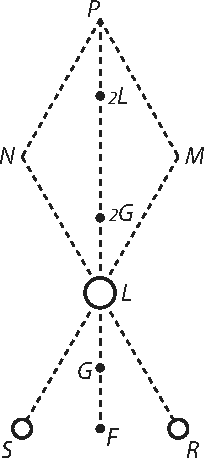
\includegraphics[width=0.21\textwidth]{%
gesamttex/edit_VIII,3/images/LH_37_05_104-105_d4_105v.pdf}}
\vspace{0.5em}
\centerline{\lbrack\textit{Fig.~4}\rbrack}
\vspace{1.5em}
%
%
\pstart%
%%%% GETRIXT:
\edtext{}{\lemma{\hspace{1,6mm}\lbrack\textit{Fig.~4}\rbrack\,}\killnumber\Cfootnote{%
Die im Text (S.~\refpassage{LH_37_05_105v_Punkte-1}{LH_37_05_105v_Punkte-2}) erwähnten Punkte \textit{{\scriptsize2}F} und \textit{{\scriptsize 2}R} sind im Diagramm nicht gezeichnet.%
}}%
Atque haec quidem
%
\edtext{recte,
ex hypothesi}{%
\lemma{recte,}\Bfootnote{%
\textit{(1)}~si ponamus
\textit{(2)}~si
\textit{(3)}~si
\textit{(4)}~ex hypothesi%
~\textit{L}}}
%
Mathematica compositi motus.%
\protect\index{Sachverzeichnis}{motus compositus}%
\protect\index{Sachverzeichnis}{hypothesis mathematica}%
\protect\index{Sachverzeichnis}{hypothesis motus compositi}
Verum in natura rerum%
\protect\index{Sachverzeichnis}{natura rerum}
talis compositio motuum%
\protect\index{Sachverzeichnis}{compositio motuum}
habet difficultates.%
\protect\index{Sachverzeichnis}{difficultas in compositione motus}
Nam a me
%
\edtext{alibi}{%
\lemma{alibi}\Cfootnote{%
Vermutlich Anspielung auf N.~\ref{RK60318} (1686 \textendash\ Oktober 1687).
	% VE2020
%Gemeint sind höchstwahrscheinlich Stücke zum schiefen Stoß in diesem Band; \textbf{welche genau}?? \textbf{Genaue Angaben wichtig}, da möglicherweise datierungsrelevant, wegen der Entwicklungen in der Theorie.
}}
%
ostensum
%
\edtext{est%
\lbrack:\rbrack\
si mobile in \textit{L} positum%
\protect\index{Sachverzeichnis}{corpus mobile}
duobus nisibus%
\protect\index{Sachverzeichnis}{nisus aequales}
aequalibus}{%
\lemma{est}\Bfootnote{%
\textit{(1)}~si corpus \textit{A} feratur
\textit{(2)}~duobus
\textit{(3)}~duobus nisibus aequ
\textit{(4)}~si mobile in
\textit{(a)}~\textit{A}
\textit{(b)}~\textit{L} positum duobus nisibus aequalibus%
~\textit{L}}}
%
feratur versus \textit{M} et versus \textit{N},
completo parallelogrammo \textit{LMPN},%
\protect\index{Sachverzeichnis}{parallelogrammum completum}
verum quidem est
corpus mobile debere moveri in diagonali \textit{LP},%
\protect\index{Sachverzeichnis}{corpus mobile}%
\protect\index{Sachverzeichnis}{diagonalis}
%
\edtext{sed dubium est
an,
%
\edtext{ut vulgo putant,%
\protect\index{Sachverzeichnis}{vulgus}%
}{%
\lemma{ut vulgo putant}\Cfootnote{%
Leibniz spielt auf die Methode an, Fälle schiefen Stoßes mithilfe der \textit{compositio motuum} zu berechnen.
Anwendungen dieser Methode (auf den schiefen Stoß zweier Körper) findet sich etwa bei E.~\textsc{Mariotte}, \textit{De la percussion}, partie II, prop.~1\textendash4 (Paris 1673, S.~179\textendash205).\cite{00311}%
}}
%
nisu seu celeritate%
\protect\index{Sachverzeichnis}{nisus seu celeritas}%
\protect\index{Sachverzeichnis}{celeritas ut diagonalis}%
\protect\index{Sachverzeichnis}{nisus ut diagonalis}
ut \textit{LP}.
\edlabel{LH_37_05_104-105_parallel_1}%
Ponamus}{%
\lemma{sed}\Bfootnote{%
\textit{(1)}~non ut ita \textlangle ut\textrangle\ eodem tem
\textit{(2)}~dubium est % an, ut vulgo putant, nisu seu celeritate 
\lbrack...\rbrack\ ut \textit{LP}.
\textit{(a)}~Sed
\textit{(b)}~Si scilicet
\textit{(c)}~Ponamus%
~\textit{L}}}
%
corpora duo%
\protect\index{Sachverzeichnis}{corpora duo impingentia}%
\protect\index{Sachverzeichnis}{concursus obliquus}
%
\edtext{aequalia}{%
\lemma{aequalia}\Bfootnote{%
\textit{erg.~L}}}
%
\textit{R} et \textit{S} impingere
eadem velocitate
eodem tempore in \textit{L},
rectis \textit{RL} et \textit{SL} % ,
quae continuatae tendant in \textit{N} et \textit{M},
et ambo quidem imprimere
%
\edtext{corpori \textit{L}
velocitates et directiones%
\protect\index{Sachverzeichnis}{velocitas impressa}%
\protect\index{Sachverzeichnis}{directio impressa}
\textit{LN} et \textit{LM}
aequales,}{%
\lemma{corpori}\Bfootnote{%
\hspace{-0,5mm}\textit{L}
\textit{(1)}~velocitatem \textit{LN} et
\textit{(2)}~velocitates et % directiones \textit{LN} et 
\lbrack...\rbrack\ \textit{LM} aequales,%
~\textit{L}}}
%
corpora autem \textit{R} et \textit{S} retinere velocitates \makebox[1.0\textwidth][s]{etiam aequales.%
\protect\index{Sachverzeichnis}{velocitas retenta}
Sint corpora \textit{L}, \textit{R}, \textit{S}
exprimenda per \textit{l}, \textit{r}, \textit{s},
et velocitas ipsius \textit{r} sit \textit{p} et}
\pend
\newpage
\centerline{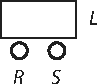
\includegraphics[width=0.12\textwidth]{%
gesamttex/edit_VIII,3/images/LH_37_05_104-105_d5_105v.pdf}}
\vspace{0.5em}
\centerline{\lbrack\textit{Fig.~5}\rbrack}%
\label{LH_37_05_105v_Fig.5}
%
%\newpage%
\vspace{1.5em}
\count\Bfootins=1200%
\count\Afootins=1200%
\count\Cfootins=1200 
\pstart
\noindent ipsius \textit{s}
%
\edtext{sit etiam \textit{p},}{%
\lemma{sit}\Bfootnote{%
\textit{(1)}~\textit{q}
\textit{(2)}~etiam \textit{p},%
~\textit{L}}}
%
erit vis ante ictum%
\protect\index{Sachverzeichnis}{vis ante ictum}
$rp^2 + sp^2,$
at velocitas impressa corpori \textit{L}%
\protect\index{Sachverzeichnis}{velocitas impressa}
%
\edtext{sit \textit{m} % ,
tam versus \textit{LN} % ,
quam versus \textit{LM},
fiet}{%
\lemma{sit}\Bfootnote{%
\hspace{-0,5mm}\textit{m},
\textit{(1)}~fiet
\textit{(2)}~fiet
\textit{(3)}~tam versus % \textit{LN}, quam versus 
\lbrack...\rbrack\ \textit{LM}, fiet%
~\textit{L}}}
%
vis ejus:%
\protect\index{Sachverzeichnis}{vis impressa}
$lm^2 + lm^2$
seu%
\protect\index{Sachverzeichnis}{vis residua}
$2lm^2,$
residua ipsorum corporum \textit{r} et \textit{s} % ,
%
\edtext{\lbrack velocitas\rbrack}{%
\lemma{vis}%
\Bfootnote{%
\textit{L~ändert Hrsg.}%
}}
%
sit \textit{q}.
Ergo fiet:
$2lm^2 + rq^2 + sq^2 = rp^2 + sp^2,$
seu
$2lm^2 = \overline{r + s} \cdot
\edtext{\overline{p^2 - q^2}.$
Ergo si
$r = s,$
fiet 
$lm^2 = r \,\overline{p^2 - q^2}.$
Sit \textit{F} centrum gr. \textit{RS}
et sit \textit{G} centr. gr.
\textit{L}\textit{R}\textit{S},
erit \textit{G} in recta \textit{FL},
et $FG : LG \,\squaredots\, l : 2r.$
Sit $FG = l,$
fiet $LG = 2r,$
quae est via centri gr. ante ictum.%
\protect\index{Sachverzeichnis}{via centri gravitatis ante ictum}%
\protect\index{Sachverzeichnis}{ictus}%
}{%
\lemma{$\overline{p^2 - q^2}$}\Bfootnote{%
\textit{(1)}~, sit \textit{p} centrum gr. \textit{RS} et
\textbar~et \textit{streicht Hrsg.}~%
\textbar\ \textit{G} sit centr. gr. \textit{LRS}, erit \textit{G} in recta \textit{FL} et \textit{LG}:
\textit{(2)}~. Ergo si % $r = s,$ fiet ...
\lbrack...\rbrack\ centr. gr. \textit{LRS},
\textit{(a)}~et
\textit{(b)}~erit \textit{G} % in recta \textit{FL}, et 
\lbrack...\rbrack\ $FG : LG \,\squaredots\, l : 2r$
\textit{(1)}~et via centri gravitatis ante ictum sit
\textit{(2)}~. Sit $FG = l$ \lbrack...\rbrack\ ante ictum.%
~\textit{L}}}
%
Cui sumenda aequalis
$L{\scriptstyle2}G = 2r,$
quae est via centri gravitatis post ictum.%
\protect\index{Sachverzeichnis}{via centri gravitatis post ictum}
Jam celeritas vera corporis \textit{L} post ictum,%
\protect\index{Sachverzeichnis}{celeritas vera post ictum}
seu recta \textit{L{\scriptsize2}L},
sit \textit{x},
fiet
${\scriptstyle2}G {\scriptstyle2}L = x -2r,$
et
%
\edtext{%
\edlabel{LH_37_05_105v_Punkte-1}%
\textit{{\scriptsize2}F{\scriptsize2}G}
ad \textit{{\scriptsize2}G{\scriptsize2}L}
ut \textit{LG} ad \textit{FG},
seu ut 2\textit{r} ad \textit{l},}{%
\lemma{\textit{{\scriptsize2}F{\scriptsize2}G} ad \lbrack...\rbrack\ ad \textit{l}}\Cfootnote{%
Leibniz verwechselt hier \textit{LG} und \textit{FG}.
Die richtige Proportion wäre:
${\scriptstyle2}F{\scriptstyle2}G : {\scriptstyle2}G{\scriptstyle2}L = FG : GL = l : 2r.$
Der Fehler wirkt sich auf die folgende Herleitung aus.%
}}
%
seu
${\scriptstyle2}F{\scriptstyle2}G : \overline{x - 2r} \,\squaredots\, 2r : l,$
seu
${\scriptstyle2}F{\scriptstyle2}G =
%
\edtext{\overline{x - 2r} \,\cdot\, 2r : l.$
Jam
%
%\edtext{}{%
%{\xxref{LH_37_05_105v_Vorzeichen-1}{LH_37_05_105v_Vorzeichen-2}}%
%{\lemma{$L{\scriptstyle2}F = {\scriptstyle2}F {\scriptstyle2}G$ \lbrack...\rbrack\ $-\, 2r\,$}\Cfootnote{%
%In der ersten Gleichung wäre $+\, L{\scriptstyle2}G$ zu erwarten, in der zweiten $+\, 2r.$}}}%
%\edlabel{LH_37_05_105v_Vorzeichen-1}%
$L{\scriptstyle2}F = {\scriptstyle2}F {\scriptstyle2}G \;\pleibvdash\, L{\scriptstyle2}G,$
erit
$L{\scriptstyle2}F = \overline{x - 2r} \cdot \overline{2r : l}\: [\pleibvdash\!]\: 2r.$%
%\edlabel{LH_37_05_105v_Vorzeichen-2}%
}{%
\lemma{$2r : l.$}\Bfootnote{%
\textit{(1)}~Jam ratio ipsius \textit{FL} ad \textit{RL}, seu ipsius
\textit{(2)}~Jam
\textit{(a)}~ratio \textit{F}
\textit{(b)}~$L{\scriptstyle2} F = {\scriptstyle2}F {\scriptstyle2}G \;\pleibvdash\, L{\scriptstyle2}G,$
\textit{(aa)}~seu
\textit{(bb)}~erit
\textit{(cc)}~erit $L{\scriptstyle2}F = \overline{x - 2r} \,\cdot\, \overline{2r : l}\
\textbar\ - \text{\textit{ändert Hrsg.}}~%
\textbar\ 2r.$%
~\textit{L}}}
%
Est autem \textit{FL} ad
%
\edtext{\textit{RL} ut $2r + l$ ad~\textit{p}.}{%
\lemma{\textit{RL}}\Bfootnote{%\hspace{-0,5mm}
\textit{(1)}~ut $2r$ ad
\textit{(2)}~seu
\textit{(3)}~ut $2r + l$ ad \textit{p}.%
~\textit{L}}}
%
Ergo et
\textit{L{\scriptsize 2}R}
seu \textit{q} ad
%
\edtext{\textit{L{\scriptsize2}F}%
\edlabel{LH_37_05_105v_Punkte-2}
ut \textit{p}
ad $2r + l,$%
}{%
\lemma{\textit{L{\scriptsize 2}F}}\Bfootnote{%\hspace{-0,5mm}
\textit{(1)}~seu ad
\textit{(2)}~ut \textit{p} ad $2r+l,$%
~\textit{L}}}
%
et fiet:
$q \cdot \overline{2r + l} = p \cdot \overline{\overline{x - 2r} \cdot \overline{2r : l} - 2r}.$
Cum ergo paulo ante habuerimus \textit{q},
tunc etiam habemus \textit{x},
sed ne implicemur calculo%
\protect\index{Sachverzeichnis}{calculus implicans}
ponamus corpori%
\protect\index{Sachverzeichnis}{corpus impactum}
%
\edtext{\lbrack\textit{L}\rbrack}{%
\lemma{\textit{R}}\Bfootnote{%
\textit{L~ändert Hrsg.}}}
%
aequaliter impingi corpora \textit{R} et \textit{S}
inter se aequalia,%
\protect\index{Sachverzeichnis}{corpora impingentia aequalia}
et ita quidem
ut post ictum quiescant ambo,%
\protect\index{Sachverzeichnis}{corpus quiescens post ictum}%
\protect\index{Sachverzeichnis}{ictus}
ipso solo pergente,%
\protect\index{Sachverzeichnis}{corpus pergens post ictum}
quod utique possibile est.
Patet non iturum corpus ea celeritate
quae sit dupla ejus
quam recepisset
si ab uno fuisset impulsum idque quiescisset,
sed
%
\edtext{\lbrack qua\rbrack}{%
\lemma{quae}\Bfootnote{%
\textit{L~ändert Hrsg.}}}
%
sit potentia dupla.%
\protect\index{Sachverzeichnis}{potentia dupla}%
\edlabel{LH_37_05_104-105_parallel_2}
\pend%
%
\pstart%
Verum
ut his tribus facilius explicemur illud%
\lbrack,\rbrack\
ajo%
\lbrack:\rbrack\
si vis centripeta%
\protect\index{Sachverzeichnis}{vis centripeta quovis momento temporis impressa}
quae quovis momento temporis%
\protect\index{Sachverzeichnis}{momentum temporis}
%%
\edtext{imprimitur,
sit ad vim insitam%
\protect\index{Sachverzeichnis}{vis insita seu viva}%
}{%
\lemma{imprimitur}\Bfootnote{%
\textit{(1)}~sit ad insitam in rati
\textit{(2)}~sit ad vim insitam%
~\textit{L}}}
%
seu
%
\edtext{vivam%
\protect\index{Sachverzeichnis}{vis viva}
incomparabiliter}{%
\lemma{vivam}\Bfootnote{%
\textit{(1)}~in est
\textit{(2)}~incomparabiliter%
~\textit{L}}}
%
parva%
\protect\index{Sachverzeichnis}{vis centripeta incomparabiliter parva}%
\lbrack,\rbrack\
nullum fieri errorem notabilem%
\protect\index{Sachverzeichnis}{error notabilis}
assumendo%
\lbrack,\rbrack\
ut positum est%
\lbrack,\rbrack\
ut areae
\textit{C{\scriptsize1}B{\scriptsize2}B}
et
\textit{C{\scriptsize2}B{\scriptsize3}B}
fieri possent aequales.%
\protect\index{Sachverzeichnis}{areae aequales}
\textlangle Sive\textrangle\
tantum difficultatis superest,%
\protect\index{Sachverzeichnis}{difficultas}
quod tunc etiam angulus fit infinite parvus,%
\protect\index{Sachverzeichnis}{angulus infinite parvus}
adeoque non nisi longissimo tempore datur curva.%
\protect\index{Sachverzeichnis}{curva data longissimo tempore}%
\protect\index{Sachverzeichnis}{tempus longissimum}
%
\edlabel{LH_37_05_105v_Vorverweis-1}%
\edtext{In genere videndum
an principium compositionis motuum%
\protect\index{Sachverzeichnis}{principium compositionis motuum}%
\protect\index{Sachverzeichnis}{compositio motuum}
servari
%
\edtext{possit%
\lbrack;\rbrack\
quid fiat}{% ,
\lemma{possit}\Bfootnote{%
\textit{(1)}~, ponendo scilicet
\textit{(2)}~quid fiat%
~\textit{L}}}
%
si corpori insolido
vi impressa%
\protect\index{Sachverzeichnis}{vis corpori insolido impressa}
pergere conanti%
\protect\index{Sachverzeichnis}{corpus vi impressa pergere conans}
semper aequalibus intervallis
corpuscula certa eodem modo imprimantur%
\protect\index{Sachverzeichnis}{corpusculum imprimens}%
\lbrack:\rbrack\
an saltem tunc sensibiliter locum habere possit
quod supponitur.
Fingenda navis.%
\protect\index{Sachverzeichnis}{navis}
Fingenda et corpora
nunc disjuncta,%
\protect\index{Sachverzeichnis}{corpora disjuncta}
nunc sese capientia.%
\protect\index{Sachverzeichnis}{corpora sese capientia}
Haec\textls{ de novo.}%
\edlabel{LH_37_05_105v_Vorverweis-2}%
}{%
\lemma{In genere \lbrack...\rbrack\ \textls{novo}}\Cfootnote{%
Wohl Vorverweis auf N.~\ref{RK60038}.
Siehe hierzu S.~\refpassage{LH_35_10_07_009-010_Datierung-1}{LH_35_10_07_009-010_Datierung-2}.}}
%
\pend%
\count\Bfootins=1200%
\count\Afootins=1200%
\count\Cfootins=1200 
%
%
%
%  %  %  %  Ende des Textes auf Blatt 105v